\documentclass{llncs}

\usepackage{graphicx}
\usepackage{amssymb}
%\usepackage[reqno]{amsmath}
\usepackage{listings}
\usepackage{url}
\usepackage{enumitem}
\usepackage{grace}
\usepackage{balance}
\usepackage{hyperref}

\author{
Sophia Drossopoulou\inst{1}
\and
James Noble\inst{2}
\and
Mark S. Miller\inst{3}
\and
Toby Murray\inst{4}
}

\institute{
Imperial College London
\email{scd@doc.ic.ac.uk}
\and
Victoria University of Wellington
\email{kjx@ecs.vuw.ac.nz}
\and
Google, Inc.\
\email{erights@google.com}
\and
{NICTA and UNSW}
\email{toby.murray@nicta.com.au}
}

\usepackage{natbib}
\usepackage{bbm}
\usepackage{framed}
\usepackage{graphics}
\definecolor{shadecolor}{rgb}{1,0.8,0.3}
%\usepackage{amsthm} % it conflicts with llncs
\usepackage{epsfig}
\usepackage{xspace}
%\usepackage{latexsym}
\usepackage{amssymb}
\usepackage{amsfonts}
%\usepackage{amstext}
% \usepackage{txfonts}
\usepackage{url}
%\usepackage{xypic}
%\usepackage{makeidx}  % allows for indexgeneration
\usepackage{listings} % for code
  \usepackage{multirow}
  \usepackage{qsymbols}
  \usepackage{amsmath}
% \usepackage{MnSymbol}


\newcommand{\prg}[1]{{\mbox{\tt{#1}}}}
\newcommand{\forget}[1]{}
\newcommand{\etc}{{\it etc.}}
\newcommand{\eg}{{\it e.g.\,}}
\newcommand{\ie}{{\it i.e.\,}}
\newcommand{\rely}{{rely}}
\newcommand{\Rely}{{Rely}}
\newcommand{\deny}{{deny}}
\newcommand{\Deny}{{Deny}}




 \newcommand{\ttt}{\prg{true}}
\newcommand{\ff}{\prg{false}}
\newcommand{\unkn}{\prg{b???}}
\newcommand{\bv}{\prg{bval}}

\newcommand{\sdparagraph}[1]{{\vspace{.3cm} \noindent \textit{#1}\ }}

\newcommand{\prg}[1]{{\mbox{\tt{#1}}}}

\newcommand{\m}{\prg{m}}
 \newcommand{\f}{\prg{f}}
  \newcommand{\e}{\prg{e}}
 \renewcommand{\c}{\prg{C}}
 \renewcommand{\v}{\prg{v}}
  \newcommand{\x}{\prg{x}}
  \newcommand{\p}{\prg{p}}
   \newcommand{\y}{\prg{y}}
      \newcommand{\uu}{\prg{u}}
  %  \newcommand{\z}{\prg{z}}
  \newcommand{\this}{\prg{this}}
  \newcommand{\caller}{\kw{caller}}
   \newcommand{\nullK}{\prg{null}}
\newcommand{\addr}{\ensuremath{\alpha}}


\newcommand{\fldMap}{\textit{fldMap}}

\newcommand{\forget}[1]{}
\newcommand{\etc}{{\it etc.}}
\newcommand{\eg}{{\it e.g.\,}}
\newcommand{\ie}{{\it i.e.\,}}

% new macros for holistic
\newcommand{\Future}[1] {\ensuremath{{\mathsf{will}}\langle \,#1\,\rangle}}
\newcommand{\Using}[2]{\ensuremath{\langle\, #1\, \mathsf{in}\, #2\, \rangle}}
\newcommand{\External}[1] {\ensuremath{{\mathsf{external}}\langle\,  #1\, \rangle}}
\newcommand{\Internal}[1] {\ensuremath{{\mathsf{internal}}\langle\,  #1\, \rangle}}
\newcommand{\Changes}[1]{\ensuremath{{\mathsf{changes}}\langle\,#1\,\rangle}}
\newcommand{\CanAccessTr}[2]{\ensuremath{\langle\, #1\, \mathsf{access}^*\, #2\, \rangle}}
\newcommand{\CanAccess}[2]{\ensuremath{\langle\, #1\, \mathsf{access}\, #2\, \rangle}}

\newcommand{\Calls}[4]{\ensuremath{\langle\, #1\, \mathsf{calls}\, #3.#2\lp#4\rp\, \rangle}}%(\!({#1})\!)}
\newcommand{\Next}[1] {\ensuremath{{\mathsf{next}}\langle \,#1\,\rangle}}%(\!({#1})\!)}
\newcommand{\PrevId}{\ensuremath{{\mathcal{P}}\textrm{\textit{rev}}}}
\newcommand{\Prev}[1] {\ensuremath{{\mathsf{prev}}\langle \,#1\,\rangle}}%(\!({#1})\!)}
\newcommand{\Past}[1]  {\ensuremath{{\mathsf{was}}\langle \,#1\,\rangle}}

\newcommand{\Name}[2]  {\ensuremath{{\mathsf{name}}\langle \,#1, #2\rangle}}

% old macros for holistic
%\newcommand{\Future}[1] 
%{{{\mathcal W}\!ill}\langle#1\rangle}%{\lozenge\, #1}% {\bullet #1}% {{{\mathcal F}}(#1)} % {{{\mathcal B}}(#1)}
%\newcommand{\Using}[2]{{\mathcal W}ith\langle\ #2,\,#1\ \rangle}
% \newcommand{\External}[1]{{\mathcal E}xternal\langle #1\rangle}
%\newcommand{\Using}[2]{#1\,{\mathcal U}sing\, #2}
%\newcommand{\Using}[2]{#1\,{\mathcal U}sing\, #2} %{{{\mathcal U}}(#1,#2)}
% \newcommand{\Changes}[1]{\ensuremath{\mathcal{C}\textrm{\textit{hange}}\langle#1\rangle}}
%\newcommand{\CanAccessTr}[2]{\ensuremath{\mathcal{A}}\textrm{\textit{ccess}}^*\langle #1,#2\rangle}
%\newcommand{\CanAccess}[2]{\ensuremath{{\mathcal{A}}\textrm{\textit{ccess}}}\langle #1,#2\rangle}%(#1,#2)}
%\newcommand{\Calls}[4]{\ensuremath{{\mathcal{C}}\textrm{\textit{alls}}}\langle #1,#2,#3,#4\rangle}%(\!({#1})\!)}
%\newcommand{\Next}[1]{\ensuremath{{\mathcal{N}}\textrm{\textit{ext}}}\langle #1\rangle}%(\!({#1})\!)}
%\newcommand{\PrevId}{\ensuremath{{\mathcal{P}}\textrm{\textit{rev}}}}
%\newcommand{\Prev}[1]{\ensuremath{{\mathcal{P}}\textrm{\textit{rev}}}\langle #1\rangle}%(\!({#1})\!)}
%\newcommand{\Caller}{\ensuremath{{\mathcal{C}}\textrm{\textit{aller}}}}

%\newcommand{\VisibleLit}{\ensuremath{\mathcal{V}\textrm{\textit{isible}}}}
%\newcommand{\Next}[1]{\ensuremath{{\mathcal{N}}\textrm{\textit{ext}}}\langle #1\rangle}%(\!({#1})\!)}
%\newcommand{\PrevId}{\ensuremath{{\mathcal{P}}\textrm{\textit{rev}}}}
%\newcommand{\Prev}[1]{\ensuremath{{\mathcal{P}}\textrm{\textit{rev}}}\langle #1\rangle}%(\!({#1})\!)}
%\newcommand{\Caller}{\ensuremath{{\mathcal{C}}\textrm{\textit{aller}}}}
% \newcommand{\Past}[1] {{{\mathcal W}\!as}\langle#1\rangle}% {\nabla #1} %{\lozenge\!\!\!\!\-\!\!-\,#1}


\newcommand{\SigmaUsing}[2]{#1\@ #2} %{{{\mathcal U}}(#1,#2)}
%{\lozenge\!\!\!\!\!\circ  #1} % {\lozenge\!\!\!\!\-\!\!- #1} %{\upupsilon #1}  %{\nabla #1} %{\circ #1}%  {{{\mathcal P}}(#1)}
\newcommand{\Initial}[1] {{{\mathcal I}\!nitial}\langle#1\rangle}

\newcommand{\Pol}[1] {{\ensuremath{\prg{Pol}\_{\prg{#1}}}}}

\newcommand{\strongImplies}{\leqq} %{{ \,^\sqsubset\!\!\!_{\sim}\, }}
\newcommand{\weakImplies}{\lessapprox} %{{ \,^\sqsubset\!\!\!_{\sim}\, }}
\newcommand{\frames}{~\kw{frames}~}

\newcommand{\appref}[1]{see App.~\ref{#1}}

\newcommand{\sE}{{\prg{e}}}
\newcommand{\varMap}{{\ensuremath{\beta}}}

\newcommand{\Lang} {\ensuremath{{\mathcal L}{_1}}}
\newcommand{\LangOO} {\ensuremath{{\mathcal L}{_{\tt {oo}}}}\xspace}
\newcommand{\Chainmail} {\ensuremath{{\mathcal C}hainmail}\xspace}

% ------------------------------------------------------------------
%                                             positions, separations
\newcommand{\cf}{{\it c.f.~}}
\newcommand{\HYPHENA}{{\em-- }}
\newcommand{\HYPHENB}{{\em-- }}
\newcommand{\SP}{{\hspace{.1in}}}
\newcommand{\s}{{\hspace{.01in}}}

\newcommand{\obeys}{\,\textbf{\textrm{obeys}}\,}
\newcommand{\StrongDom}{\ensuremath{\mathcal{S}\textrm{\textit{trong}}{\mathcal{D}}\textrm{\textit{om}}}}
\newcommand{\Dom}{\ensuremath{\mathcal{D}}\textrm{\textit{om}}}


\newcommand{\Gives}{\ensuremath{\mathcal{G}\textrm{\textit{ives}}}}
%{\ensuremath{\mathcal{C}\textrm{\textit{an}}{\mathcal{A}}\textrm{\textit{ccess}}}(#1,#2)}
\newcommand{\A}{\ensuremath{A}}
\newcommand{\B}{\ensuremath{B}}
\newcommand{\Arising}[1]{{\mathcal{A}}\textrm{\textit{rising}}(#1)}

 %------------------------ syntax tables

\newcommand{\syntax}[1]{\prg{{\it #1}}}
\newcommand{\BBC}{$::=$} %in syntactic definitions
\newcommand{\SOR}{\ensuremath{\ \mid\ }} % BNF or
\newcommand{\MID}{{\SPsmall ~ \mid ~ \SPsmall }} % in sets


\newcommand{\pre}{\ensuremath{_{{pre}}}}   %kjx no \sc  in math mode
\newcommand{\post}{\ensuremath{_{{post}}}} %kjx no \sc  in math mode
\newcommand{\PRE}{\pre}
\newcommand{\POST}{\post}

 \newcommand{\interp}[2]{{\ensuremath{\lfloor{ {#1}}\rfloor_{#2}}}}
% \newcommand{\interpBL}[1]{{\lceil   {#1}  \rfloor}}

% ------------------------------------------------------------------
%                                              keywords, program text
\newcommand{\kw}[1]{\prg{#1}} % {{\bf{\sf {#1}}}}
\newcommand{\kwN}[1]{{\bf{\sf {#1}}}}
\newcommand{\returnKW}{{\bf{\sf {return}}}}
\newcommand{\newKW}{\mbox{\bf{\sf{new}}}}

\newcommand{\lit}[1]{{\prg {#1}\xspace}}
\newcommand{\com}{\ensuremath{\prg{//}}}


\newcommand{\ass}{\mbox{{\kw {:=}}\,}}
\newcommand{\semi}{\mbox{{\kw {;}}\ }}
\newcommand{\comma}{\mbox{{\kw {,}}\,}}
\newcommand{\lb}{\prg{\mbox{\tt{\bf{\{ }}}}}
\newcommand{\rb}{\prg{\mbox{\tt{\bf{\} }}}}}
\newcommand{\lp}{\prg{\mbox{\tt{\bf{( }}}}}
\newcommand{\rp}{\prg{\mbox{\tt{\bf{) }}}}}
%\newcommand{\thisL}{{\lit {this}}}% no~around it
\newcommand{\nullKW}{{\lit {null}}~}
\newcommand{\true}{{\lit {true}}~}
\newcommand{\false}{{\lit {false}}~}
\newcommand{\return}{{\kw {return}}\s}

 \newcommand{\M}{\prg{\ensuremath{\prg{M}}}}
  \newcommand{\Prog}[1]{\M{#1}}

\newcommand{\mkpair}{\fatsemi}
\newcommand{\subconf}{\ensuremath{\sqsubseteq}}
\newcommand{\restrct}[2]{\ensuremath{#1\!\!\downarrow\!_{#2}}}
\newcommand{\adapt}{\ensuremath{\!\triangleleft\!}}
\newcommand{\link}{\!\circ\!}

\newcommand{\ClassOf}[2] {\ensuremath{{\mathcal C}{\mathit{lass}}(#1)_{#2}}}

% --- assertions and expressions - simple

\newcommand{\SA}{\ensuremath{B}}%{\ensuremath{\prg{B}}}
\newcommand{\SAPrime}{\ensuremath{B'}}

\newcommand{\SE}{\ensuremath{\prg{e}}}
\newcommand{\SEPrime}{\ensuremath{\prg{e}'}}
\newcommand{\SEOne}{\ensuremath{\prg{e}_1}}
\newcommand{\SETwo}{\ensuremath{\prg{e}_2}}




%\newcommand{\Prog}[1]  {{\ensuremath{\prg{M}{{\prg{#1}}}}}}
    % {\prg{P}}

\newcommand{\expandexp}[1]{}

\newcommand{\oo}{object-oriented}
\newcommand{\mExtS}{\ensuremath{\Downarrow}}

% re-classification expression
\newcommand{\cm}[1]{\this{\prg{\ensuremath{\mExtS}}}\prg{#1}}

\newcommand{\refDef}[1]{Definition \ref{{#1}}}

% structuring macros
\newcommand{\EndDefLemma}{\noindent $\bigtriangleup$}

 %-------------------- implies, and, or, iff, etc -----------------
  \newcommand{\AND}{{\SPsmall {\mbox{and}} \SPsmall}}
\newcommand{\WITH}{{\SPsmall {\mbox{with}} \SPsmall}}
 \newcommand{\IFF}{{\SP {\mbox{ if }} \SP}}
\newcommand{\OR}{{\SPsmall {\mbox{or}} \SPsmall}}
%\newcommand{\implies}{{\ensuremath{\longrightarrow}}}
\newcommand{\upd}{{\mapsto}}

\newcommand{\SAF}{\ensuremath{W}} % {\prg{AFs}}






%Macros for inference rules
\newcommand{\inferencerule}[2]{
\begin{array}{l} #1 \\ \hline #2 \end{array}
}


\newcommand{\inferenceruleExact}[4]
{
\begin{array}{l}
{#1}  {\sf #2}
\\ #3  \\ \hline   #4
  \end{array}
}

\newcommand{\inferenceruleN}[3]
{
\begin{array}{l}
%\SP\SP\SP\SP\SP\SP\SP\SP
\SP\SP\SP\SP\SP  {\sf #1}
\\ #2  \\ \hline   #3
  \end{array}
}

\newcommand{\inferenceruleNM}[3]
{
\begin{array}{l}
\SP\SP\SP\SP\SP \SP\SP\SP\SP\SP\SP\SP\SP  {\sf #1}
\\ #2  \\ \hline   #3
  \end{array}
}

\newcommand{\inferenceruleNN}[3]
{
\begin{array}{l}
\SP\SP\SP\SP\SP\SP\SP\SP
\SP\SP\SP\SP\SP\SP\SP\SP
\SP\SP\SP\SP\SP\SP\SP\SP
\SP\SP\SP\SP\SP\SP\SP\SP
\SP\SP\SP\SP\SP\SP\SP\SP
\SP\SP
   {\sf #1}
\\ #2  \\ \hline   #3
  \end{array}
}

%===========================================================================
%  Definition-Lemma-Theorem-Proof
%
% Adaptation of LaTeX's theorem environment; can be used as a command
% (eg just \Lemma not \begin{Lemma}) and no italicisation; also works
% with ptmac; result numbering is uniform within subsections and can be
% suppressed.
%
\newif\ifNumberResults\NumberResultstrue
\def\@@opargbegintheorem#1#2#3{\@@@@begintheorem{\bf\@@thmname{#1}{#2}(#3)}}
\def\@@begintheorem#1#2{\@@@@begintheorem{\bf\@@thmname{#1}{#2}}}
\def\@@@@begintheorem#1{\par\removelastskip\smallskip\noindent{#1}}
\def\@@thmname#1#2{#1\ \ifNumberResults#2\ \fi}

% similarly \Proof or \begin{Proof}...\end{Proof}
% prefer proofs with statements if possible - hence \penalty700
%\let\qedsymbol\S% make it \square or \blacksquare if you like for kb
\let\qedsymbol \Box
\def\qed{\hfill{$\qedsymbol$}}
\def\Proof{\par\removelastskip\smallskip\penalty700\noindent{\bf Proof}\enskip}
\def\endProof{\qed\penalty-700 \smallskip}
\let\endproof\endProof

%   The actual words

\newtheorem{theo}{Theorem}
\newtheorem{definition}[theo]{Definition}
%\newtheorem{example}[theo]{Example}
\newtheorem{mylemma}[theo]{Lemma}
%\newtheorem{conjecture}[theo]{Conjecture}
% \newtheorem{theorem}{Theorem}
% \newtheorem{note}[theo]{Note}
 \newtheorem{observation}[theo]{Observation}


%--------------------------------- the ones that Susan introduced
\newcommand{\SF}{{\prg S}}
\newcommand{\z}{{\prg z}}
\newcommand{\pu}{{\prg u}}
\newcommand{\pb}{{\prg b}}
\newcommand{\acc}{{\prg a}}
\newcommand{\bal}{{\prg{balance}}}
\newcommand{\zs}{{\prg{zs}}}

\newcommand{\Fields}[3]{\ensuremath{{\mathcal F}(}\Prog{#1},\prg{#2},
\prg{#3}\ensuremath{)} }
\newcommand{\FieldIds}[2]{\ensuremath{{\mathcal F}{\it {s}}(\Prog{#1},\prg{#2})}}
\newcommand{\Meths}[3]{\ensuremath{{\mathcal M}(}\Prog{#1},\prg{#2},
\prg{#3}\ensuremath{)} }





\newcommand{\WideFig}[3]
{
\begin{figure*}[t]
\begin{center}
\noindent
\fbox{
\begin{minipage}{4.7 in}
{#1} % the contents
\end{minipage}
}
\caption{#2}
\label{#3}
\end{center}
\end{figure*}
}


\newcommand{\WideFigWhere}[4] % you can specify where it should appear!
{
\begin{figure*}[{#4}]
\begin{center}
\noindent
\fbox{
\begin{minipage}{5. in}
{#1} % the contents
\end{minipage}
}
\caption{#2}
\label{#3}
\end{center}
\end{figure*}
}

\newcommand{\BigWideFigWhere}[4] % you can specify where it should appear!
{
\begin{figure*}[{#4}]
\begin{center}
\noindent
{\normalsize
\hrule
\begin{minipage}{5. in}
{#1} % the contents
\end{minipage}
\hrule
}
\caption{#2}
\label{#3}
\end{center}
\end{figure*}
}

\newcommand{\NotTooWideFigWhere}[4] % you can specify where it should appear!
{
\begin{figure*}[{#4}]
\begin{center}
\noindent
\fbox{
\begin{minipage}{4.3 in}
{#1} % the contents
\end{minipage}
}
\caption{#2}
\label{#3}
\end{center}
\end{figure*}
}


\newcommand{\opsemExprFig}
{\BigWideFigWhere {\opsemExpr} {Execution of expressions\MD}
{opsemTrad} {htbp} }



\newcommand{\mlc}{ }%{\heartsuit}
%\newcommand{\mcl}{ }%{\heartsuit}
\newcommand{\mc}{ }%{\heartsuit}

\newcommand{\BigNotTooWideFigWhere}[4] % you can specify where it should appear!
{
\begin{figure*}[{#4}]
\begin{center}
\noindent
{\normalsize
\hrule
\begin{minipage}{4.3 in}
{#1} % the contents
\end{minipage}
\hrule
}
\caption{#2}
\label{#3}
\end{center}
\end{figure*}
}

 \newcommand{\hlc}[2][yellow]{{%
    \colorlet{foo}{#1}%
    \sethlcolor{foo}\hl{#2}}%\prg{m}''
}

%]})
%}



\usepackage{times}
\usepackage{latexsym}
\usepackage{listings}
\definecolor{dkgreen}{rgb}{0,0.6,0}
\definecolor{gray}{rgb}{0.5,0.5,0.5}
\definecolor{mauve}{rgb}{0.58,0,0.82}


\lstset{ %
  language=Java,                % the language of the code
  mathescape=true,
  basicstyle=\footnotesize\tt,           % the size of the fonts that are used for the code
  numbers=left,                   % where to put the line-numbers
  numberstyle=\tiny\color{dkgreen},  % the style that is used for the line-numbers
  stepnumber=1,                   % the step between two line-numbers. If it's 1, each line
                                  % will be numbered
  numbersep=5pt,                  % how far the line-numbers are from the code
  backgroundcolor=\color{white},      % choose the background color. You must add \usepackage{color}
  showspaces=false,               % show spaces adding particular underscores
  showstringspaces=false,         % underline spaces within strings
  showtabs=false,                 % show tabs within strings adding particular underscores
  frame=single,                   % adds a frame around the code
  rulecolor=\color{black},        % if not set, the frame-color may be changed on line-breaks within not-black text (e.g. commens (green here))
  tabsize=2,                      % sets default tabsize to 2 spaces
  captionpos=b,                   % sets the caption-position to bottom
  breaklines=true,                % sets automatic line breaking
  breakatwhitespace=false,        % sets if automatic breaks should only happen at whitespace
  title=\lstname,                   % show the filename of files included with \lstinputlisting;
                                  % also try caption instead of title
  keywordstyle=\color{blue},          % keyword style
  commentstyle=\color{gray},       % comment style
  stringstyle=\color{mauve},         % string literal style
  escapeinside={\%*}{*)},            % if you want to add LaTeX within your code
  morekeywords={field,fields,predicate,private,public,final,this,throw,new,||,to,method,def,any,specification,policies,policy,then,where}               % if you want to add more keywords to the set
}


% \newcommand{\ttt}{\prg{true}}
\newcommand{\ff}{\prg{false}}
\newcommand{\unkn}{\prg{b???}}
\newcommand{\bv}{\prg{bval}}

\newcommand{\sdparagraph}[1]{{\vspace{.3cm} \noindent \textit{#1}\ }}

\newcommand{\prg}[1]{{\mbox{\tt{#1}}}}

\newcommand{\m}{\prg{m}}
 \newcommand{\f}{\prg{f}}
  \newcommand{\e}{\prg{e}}
 \renewcommand{\c}{\prg{C}}
 \renewcommand{\v}{\prg{v}}
  \newcommand{\x}{\prg{x}}
  \newcommand{\p}{\prg{p}}
   \newcommand{\y}{\prg{y}}
      \newcommand{\uu}{\prg{u}}
  %  \newcommand{\z}{\prg{z}}
  \newcommand{\this}{\prg{this}}
  \newcommand{\caller}{\kw{caller}}
   \newcommand{\nullK}{\prg{null}}
\newcommand{\addr}{\ensuremath{\alpha}}


\newcommand{\fldMap}{\textit{fldMap}}

\newcommand{\forget}[1]{}
\newcommand{\etc}{{\it etc.}}
\newcommand{\eg}{{\it e.g.\,}}
\newcommand{\ie}{{\it i.e.\,}}

% new macros for holistic
\newcommand{\Future}[1] {\ensuremath{{\mathsf{will}}\langle \,#1\,\rangle}}
\newcommand{\Using}[2]{\ensuremath{\langle\, #1\, \mathsf{in}\, #2\, \rangle}}
\newcommand{\External}[1] {\ensuremath{{\mathsf{external}}\langle\,  #1\, \rangle}}
\newcommand{\Internal}[1] {\ensuremath{{\mathsf{internal}}\langle\,  #1\, \rangle}}
\newcommand{\Changes}[1]{\ensuremath{{\mathsf{changes}}\langle\,#1\,\rangle}}
\newcommand{\CanAccessTr}[2]{\ensuremath{\langle\, #1\, \mathsf{access}^*\, #2\, \rangle}}
\newcommand{\CanAccess}[2]{\ensuremath{\langle\, #1\, \mathsf{access}\, #2\, \rangle}}

\newcommand{\Calls}[4]{\ensuremath{\langle\, #1\, \mathsf{calls}\, #3.#2\lp#4\rp\, \rangle}}%(\!({#1})\!)}
\newcommand{\Next}[1] {\ensuremath{{\mathsf{next}}\langle \,#1\,\rangle}}%(\!({#1})\!)}
\newcommand{\PrevId}{\ensuremath{{\mathcal{P}}\textrm{\textit{rev}}}}
\newcommand{\Prev}[1] {\ensuremath{{\mathsf{prev}}\langle \,#1\,\rangle}}%(\!({#1})\!)}
\newcommand{\Past}[1]  {\ensuremath{{\mathsf{was}}\langle \,#1\,\rangle}}

\newcommand{\Name}[2]  {\ensuremath{{\mathsf{name}}\langle \,#1, #2\rangle}}

% old macros for holistic
%\newcommand{\Future}[1] 
%{{{\mathcal W}\!ill}\langle#1\rangle}%{\lozenge\, #1}% {\bullet #1}% {{{\mathcal F}}(#1)} % {{{\mathcal B}}(#1)}
%\newcommand{\Using}[2]{{\mathcal W}ith\langle\ #2,\,#1\ \rangle}
% \newcommand{\External}[1]{{\mathcal E}xternal\langle #1\rangle}
%\newcommand{\Using}[2]{#1\,{\mathcal U}sing\, #2}
%\newcommand{\Using}[2]{#1\,{\mathcal U}sing\, #2} %{{{\mathcal U}}(#1,#2)}
% \newcommand{\Changes}[1]{\ensuremath{\mathcal{C}\textrm{\textit{hange}}\langle#1\rangle}}
%\newcommand{\CanAccessTr}[2]{\ensuremath{\mathcal{A}}\textrm{\textit{ccess}}^*\langle #1,#2\rangle}
%\newcommand{\CanAccess}[2]{\ensuremath{{\mathcal{A}}\textrm{\textit{ccess}}}\langle #1,#2\rangle}%(#1,#2)}
%\newcommand{\Calls}[4]{\ensuremath{{\mathcal{C}}\textrm{\textit{alls}}}\langle #1,#2,#3,#4\rangle}%(\!({#1})\!)}
%\newcommand{\Next}[1]{\ensuremath{{\mathcal{N}}\textrm{\textit{ext}}}\langle #1\rangle}%(\!({#1})\!)}
%\newcommand{\PrevId}{\ensuremath{{\mathcal{P}}\textrm{\textit{rev}}}}
%\newcommand{\Prev}[1]{\ensuremath{{\mathcal{P}}\textrm{\textit{rev}}}\langle #1\rangle}%(\!({#1})\!)}
%\newcommand{\Caller}{\ensuremath{{\mathcal{C}}\textrm{\textit{aller}}}}

%\newcommand{\VisibleLit}{\ensuremath{\mathcal{V}\textrm{\textit{isible}}}}
%\newcommand{\Next}[1]{\ensuremath{{\mathcal{N}}\textrm{\textit{ext}}}\langle #1\rangle}%(\!({#1})\!)}
%\newcommand{\PrevId}{\ensuremath{{\mathcal{P}}\textrm{\textit{rev}}}}
%\newcommand{\Prev}[1]{\ensuremath{{\mathcal{P}}\textrm{\textit{rev}}}\langle #1\rangle}%(\!({#1})\!)}
%\newcommand{\Caller}{\ensuremath{{\mathcal{C}}\textrm{\textit{aller}}}}
% \newcommand{\Past}[1] {{{\mathcal W}\!as}\langle#1\rangle}% {\nabla #1} %{\lozenge\!\!\!\!\-\!\!-\,#1}


\newcommand{\SigmaUsing}[2]{#1\@ #2} %{{{\mathcal U}}(#1,#2)}
%{\lozenge\!\!\!\!\!\circ  #1} % {\lozenge\!\!\!\!\-\!\!- #1} %{\upupsilon #1}  %{\nabla #1} %{\circ #1}%  {{{\mathcal P}}(#1)}
\newcommand{\Initial}[1] {{{\mathcal I}\!nitial}\langle#1\rangle}

\newcommand{\Pol}[1] {{\ensuremath{\prg{Pol}\_{\prg{#1}}}}}

\newcommand{\strongImplies}{\leqq} %{{ \,^\sqsubset\!\!\!_{\sim}\, }}
\newcommand{\weakImplies}{\lessapprox} %{{ \,^\sqsubset\!\!\!_{\sim}\, }}
\newcommand{\frames}{~\kw{frames}~}

\newcommand{\appref}[1]{see App.~\ref{#1}}

\newcommand{\sE}{{\prg{e}}}
\newcommand{\varMap}{{\ensuremath{\beta}}}

\newcommand{\Lang} {\ensuremath{{\mathcal L}{_1}}}
\newcommand{\LangOO} {\ensuremath{{\mathcal L}{_{\tt {oo}}}}\xspace}
\newcommand{\Chainmail} {\ensuremath{{\mathcal C}hainmail}\xspace}

% ------------------------------------------------------------------
%                                             positions, separations
\newcommand{\cf}{{\it c.f.~}}
\newcommand{\HYPHENA}{{\em-- }}
\newcommand{\HYPHENB}{{\em-- }}
\newcommand{\SP}{{\hspace{.1in}}}
\newcommand{\s}{{\hspace{.01in}}}

\newcommand{\obeys}{\,\textbf{\textrm{obeys}}\,}
\newcommand{\StrongDom}{\ensuremath{\mathcal{S}\textrm{\textit{trong}}{\mathcal{D}}\textrm{\textit{om}}}}
\newcommand{\Dom}{\ensuremath{\mathcal{D}}\textrm{\textit{om}}}


\newcommand{\Gives}{\ensuremath{\mathcal{G}\textrm{\textit{ives}}}}
%{\ensuremath{\mathcal{C}\textrm{\textit{an}}{\mathcal{A}}\textrm{\textit{ccess}}}(#1,#2)}
\newcommand{\A}{\ensuremath{A}}
\newcommand{\B}{\ensuremath{B}}
\newcommand{\Arising}[1]{{\mathcal{A}}\textrm{\textit{rising}}(#1)}

 %------------------------ syntax tables

\newcommand{\syntax}[1]{\prg{{\it #1}}}
\newcommand{\BBC}{$::=$} %in syntactic definitions
\newcommand{\SOR}{\ensuremath{\ \mid\ }} % BNF or
\newcommand{\MID}{{\SPsmall ~ \mid ~ \SPsmall }} % in sets


\newcommand{\pre}{\ensuremath{_{{pre}}}}   %kjx no \sc  in math mode
\newcommand{\post}{\ensuremath{_{{post}}}} %kjx no \sc  in math mode
\newcommand{\PRE}{\pre}
\newcommand{\POST}{\post}

 \newcommand{\interp}[2]{{\ensuremath{\lfloor{ {#1}}\rfloor_{#2}}}}
% \newcommand{\interpBL}[1]{{\lceil   {#1}  \rfloor}}

% ------------------------------------------------------------------
%                                              keywords, program text
\newcommand{\kw}[1]{\prg{#1}} % {{\bf{\sf {#1}}}}
\newcommand{\kwN}[1]{{\bf{\sf {#1}}}}
\newcommand{\returnKW}{{\bf{\sf {return}}}}
\newcommand{\newKW}{\mbox{\bf{\sf{new}}}}

\newcommand{\lit}[1]{{\prg {#1}\xspace}}
\newcommand{\com}{\ensuremath{\prg{//}}}


\newcommand{\ass}{\mbox{{\kw {:=}}\,}}
\newcommand{\semi}{\mbox{{\kw {;}}\ }}
\newcommand{\comma}{\mbox{{\kw {,}}\,}}
\newcommand{\lb}{\prg{\mbox{\tt{\bf{\{ }}}}}
\newcommand{\rb}{\prg{\mbox{\tt{\bf{\} }}}}}
\newcommand{\lp}{\prg{\mbox{\tt{\bf{( }}}}}
\newcommand{\rp}{\prg{\mbox{\tt{\bf{) }}}}}
%\newcommand{\thisL}{{\lit {this}}}% no~around it
\newcommand{\nullKW}{{\lit {null}}~}
\newcommand{\true}{{\lit {true}}~}
\newcommand{\false}{{\lit {false}}~}
\newcommand{\return}{{\kw {return}}\s}

 \newcommand{\M}{\prg{\ensuremath{\prg{M}}}}
  \newcommand{\Prog}[1]{\M{#1}}

\newcommand{\mkpair}{\fatsemi}
\newcommand{\subconf}{\ensuremath{\sqsubseteq}}
\newcommand{\restrct}[2]{\ensuremath{#1\!\!\downarrow\!_{#2}}}
\newcommand{\adapt}{\ensuremath{\!\triangleleft\!}}
\newcommand{\link}{\!\circ\!}

\newcommand{\ClassOf}[2] {\ensuremath{{\mathcal C}{\mathit{lass}}(#1)_{#2}}}

% --- assertions and expressions - simple

\newcommand{\SA}{\ensuremath{B}}%{\ensuremath{\prg{B}}}
\newcommand{\SAPrime}{\ensuremath{B'}}

\newcommand{\SE}{\ensuremath{\prg{e}}}
\newcommand{\SEPrime}{\ensuremath{\prg{e}'}}
\newcommand{\SEOne}{\ensuremath{\prg{e}_1}}
\newcommand{\SETwo}{\ensuremath{\prg{e}_2}}




%\newcommand{\Prog}[1]  {{\ensuremath{\prg{M}{{\prg{#1}}}}}}
    % {\prg{P}}

\newcommand{\expandexp}[1]{}

\newcommand{\oo}{object-oriented}
\newcommand{\mExtS}{\ensuremath{\Downarrow}}

% re-classification expression
\newcommand{\cm}[1]{\this{\prg{\ensuremath{\mExtS}}}\prg{#1}}

\newcommand{\refDef}[1]{Definition \ref{{#1}}}

% structuring macros
\newcommand{\EndDefLemma}{\noindent $\bigtriangleup$}

 %-------------------- implies, and, or, iff, etc -----------------
  \newcommand{\AND}{{\SPsmall {\mbox{and}} \SPsmall}}
\newcommand{\WITH}{{\SPsmall {\mbox{with}} \SPsmall}}
 \newcommand{\IFF}{{\SP {\mbox{ if }} \SP}}
\newcommand{\OR}{{\SPsmall {\mbox{or}} \SPsmall}}
%\newcommand{\implies}{{\ensuremath{\longrightarrow}}}
\newcommand{\upd}{{\mapsto}}

\newcommand{\SAF}{\ensuremath{W}} % {\prg{AFs}}






%Macros for inference rules
\newcommand{\inferencerule}[2]{
\begin{array}{l} #1 \\ \hline #2 \end{array}
}


\newcommand{\inferenceruleExact}[4]
{
\begin{array}{l}
{#1}  {\sf #2}
\\ #3  \\ \hline   #4
  \end{array}
}

\newcommand{\inferenceruleN}[3]
{
\begin{array}{l}
%\SP\SP\SP\SP\SP\SP\SP\SP
\SP\SP\SP\SP\SP  {\sf #1}
\\ #2  \\ \hline   #3
  \end{array}
}

\newcommand{\inferenceruleNM}[3]
{
\begin{array}{l}
\SP\SP\SP\SP\SP \SP\SP\SP\SP\SP\SP\SP\SP  {\sf #1}
\\ #2  \\ \hline   #3
  \end{array}
}

\newcommand{\inferenceruleNN}[3]
{
\begin{array}{l}
\SP\SP\SP\SP\SP\SP\SP\SP
\SP\SP\SP\SP\SP\SP\SP\SP
\SP\SP\SP\SP\SP\SP\SP\SP
\SP\SP\SP\SP\SP\SP\SP\SP
\SP\SP\SP\SP\SP\SP\SP\SP
\SP\SP
   {\sf #1}
\\ #2  \\ \hline   #3
  \end{array}
}

%===========================================================================
%  Definition-Lemma-Theorem-Proof
%
% Adaptation of LaTeX's theorem environment; can be used as a command
% (eg just \Lemma not \begin{Lemma}) and no italicisation; also works
% with ptmac; result numbering is uniform within subsections and can be
% suppressed.
%
\newif\ifNumberResults\NumberResultstrue
\def\@@opargbegintheorem#1#2#3{\@@@@begintheorem{\bf\@@thmname{#1}{#2}(#3)}}
\def\@@begintheorem#1#2{\@@@@begintheorem{\bf\@@thmname{#1}{#2}}}
\def\@@@@begintheorem#1{\par\removelastskip\smallskip\noindent{#1}}
\def\@@thmname#1#2{#1\ \ifNumberResults#2\ \fi}

% similarly \Proof or \begin{Proof}...\end{Proof}
% prefer proofs with statements if possible - hence \penalty700
%\let\qedsymbol\S% make it \square or \blacksquare if you like for kb
\let\qedsymbol \Box
\def\qed{\hfill{$\qedsymbol$}}
\def\Proof{\par\removelastskip\smallskip\penalty700\noindent{\bf Proof}\enskip}
\def\endProof{\qed\penalty-700 \smallskip}
\let\endproof\endProof

%   The actual words

\newtheorem{theo}{Theorem}
\newtheorem{definition}[theo]{Definition}
%\newtheorem{example}[theo]{Example}
\newtheorem{mylemma}[theo]{Lemma}
%\newtheorem{conjecture}[theo]{Conjecture}
% \newtheorem{theorem}{Theorem}
% \newtheorem{note}[theo]{Note}
 \newtheorem{observation}[theo]{Observation}


%--------------------------------- the ones that Susan introduced
\newcommand{\SF}{{\prg S}}
\newcommand{\z}{{\prg z}}
\newcommand{\pu}{{\prg u}}
\newcommand{\pb}{{\prg b}}
\newcommand{\acc}{{\prg a}}
\newcommand{\bal}{{\prg{balance}}}
\newcommand{\zs}{{\prg{zs}}}

\newcommand{\Fields}[3]{\ensuremath{{\mathcal F}(}\Prog{#1},\prg{#2},
\prg{#3}\ensuremath{)} }
\newcommand{\FieldIds}[2]{\ensuremath{{\mathcal F}{\it {s}}(\Prog{#1},\prg{#2})}}
\newcommand{\Meths}[3]{\ensuremath{{\mathcal M}(}\Prog{#1},\prg{#2},
\prg{#3}\ensuremath{)} }





\newcommand{\WideFig}[3]
{
\begin{figure*}[t]
\begin{center}
\noindent
\fbox{
\begin{minipage}{4.7 in}
{#1} % the contents
\end{minipage}
}
\caption{#2}
\label{#3}
\end{center}
\end{figure*}
}


\newcommand{\WideFigWhere}[4] % you can specify where it should appear!
{
\begin{figure*}[{#4}]
\begin{center}
\noindent
\fbox{
\begin{minipage}{5. in}
{#1} % the contents
\end{minipage}
}
\caption{#2}
\label{#3}
\end{center}
\end{figure*}
}

\newcommand{\BigWideFigWhere}[4] % you can specify where it should appear!
{
\begin{figure*}[{#4}]
\begin{center}
\noindent
{\normalsize
\hrule
\begin{minipage}{5. in}
{#1} % the contents
\end{minipage}
\hrule
}
\caption{#2}
\label{#3}
\end{center}
\end{figure*}
}

\newcommand{\NotTooWideFigWhere}[4] % you can specify where it should appear!
{
\begin{figure*}[{#4}]
\begin{center}
\noindent
\fbox{
\begin{minipage}{4.3 in}
{#1} % the contents
\end{minipage}
}
\caption{#2}
\label{#3}
\end{center}
\end{figure*}
}


\newcommand{\opsemExprFig}
{\BigWideFigWhere {\opsemExpr} {Execution of expressions\MD}
{opsemTrad} {htbp} }



\newcommand{\mlc}{ }%{\heartsuit}
%\newcommand{\mcl}{ }%{\heartsuit}
\newcommand{\mc}{ }%{\heartsuit}

\newcommand{\BigNotTooWideFigWhere}[4] % you can specify where it should appear!
{
\begin{figure*}[{#4}]
\begin{center}
\noindent
{\normalsize
\hrule
\begin{minipage}{4.3 in}
{#1} % the contents
\end{minipage}
\hrule
}
\caption{#2}
\label{#3}
\end{center}
\end{figure*}
}

 \newcommand{\hlc}[2][yellow]{{%
    \colorlet{foo}{#1}%
    \sethlcolor{foo}\hl{#2}}%\prg{m}''
}

%]})
%}

\usepackage{enumitem}
\setlist{nolistsep}


\renewcommand\floatpagefraction{1}
\renewcommand\dblfloatpagefraction{1}
\renewcommand{\textfraction}{0.07}
\renewcommand{\topfraction}{0.9}
\newcommand{\definitionautorefname}{Definition}
\renewcommand{\theoremautorefname}{Theorem}
\newcommand{\lemmaautorefname}{Lemma}
\renewcommand{\sectionautorefname}{Section}
\renewcommand{\subsectionautorefname}{Section}
\renewcommand{\subsubsectionautorefname}{Section}

\begin{document}

\pagestyle{plain}

 \title{Reasoning about Risk and Trust in an Open Word}


% \subtitle{First Steps towards Reasoning about Risk and Trust in an Open World}
%\subtitle{Reasoning about Object Capabilities in an Open World}

\maketitle

\begin{abstract}
  Contemporary open systems use components developed by % many
  different parties, linked together dynamically in unforeseen
  constellations.  Code needs to live up to strict {\em security
    requirements}, and ensure the correct functioning of its objects
  even when they collaborate with external, potentially malicious,
  objects.

  In this paper we propose special specification predicates that model
  risk and trust in open systems.  We specify Miller, Van Cutsem, and
  Tulloh's escrow exchange example, and discuss the meaning of such a
  specification.

%  We propose special predicates which model trust and risk.
%James likes the last sentence or something
% SD I like it too, but I think it no longer fits!
%  By modelling risk and trust explicitly, we show how to reason
%  about security specifications in an open world.

  \jn{We propose a novel Hoare logic, based on four-tuples, including
    an invariant describing properties preserved by the execution of a
    statement as well as a postcondition describing the state after
    execution.
%
  We model specification and programing languages based on the
  Hoare logic, prove soundness, and
  prove the key steps of the Escrow protocol.}
\end{abstract}


\section{Necessary Conditions and Robustness}
\label{s:intro}

%\subsection{Necessary conditions and Robustness}

%% Today's   software has been built 
%% over decades by combining modules and components of
%% different provenance and 
%% %different degrees of 
%% trustworthiness, and
%% is \emph{open}, interacting with other programs, devices, and people.

% according to IEEE standard,
% robust = The degree to which a system or component can function correctly in the presence 
% of invalid inputs or stressful environmental conditions.  

{Software needs} to be both {\emph{correct}} ({programs do what they
  are supposed to}) and {\emph{robust}} ({programs only do what
  they're supposed to}). Robustness means that
programs don't do what they aren't supposed to do, even in the
presence of untrusted or malicious {clients} \cite{ieeeStandard}.
% robust = The degree to which a system or component can function correctly in the presence 
% of invalid inputs or stressful environmental conditions.  
{Correctness is} \jm[]{traditionally} specified
%formally 
through \citeasnoun{Hoare69} triples: a  precondition, a code snippet, and a
 postcondition. 
 For example,  {part of the \funcSpec
   of a \prg{transfer} method for a bank module is that the source account's balance decreases:}
 \begin{quote}
   \Scorrect\ \ $\triangleq$  
 % SD I could not make the below work ...
 % {\scriptsize \lstinline*{pwd=src.pwd  $\wedge$ \lstinline* src.bal=b} src.transfer(dst,pwd) {src.bal=b-100 * $\wedge$ \ldots } } }\\
 {\footnotesize{ $\{\,$\prg{pwd=src.pwd} $\,\wedge\,$ \prg{src.bal=b}$\,\}$ \prg{src.transfer(dst,pwd)} $\{$ \prg{src.bal=b-100}$\,\wedge\,\dots \}$ }} Calling \prg{transfer} on  {an account with the correct password} will transfer the money.
\end{quote}
Assuming termination, the precondition is a \emph{sufficient} condition for the {code snippet to behave correctly}: 
%assuming termination, 
the precondition (\eg providing the right 
password) guarantees that
the code (\eg call the \prg{transfer} function)
will always achieve the postcondition (the money is transferred).
 
    \vspace{.05in}
    % I think we need the vspace
 
%While 
\Scorrect  describes  {the \emph{correct use} of the module, but is \emph{not} concerned with its \emph{robustness}.}
{For example, can I pass an account to foreign untrusted code, in the expectation of receiving a payment,
but without fear that a malicious client might use the account to steal my money \cite{ELang}?}
 A first \jm[]{attempt} to specify robustness could be:
 

\begin{quote}
\SrobustA\ \ $\triangleq$ \ \ An account's balance does not decrease unless \prg{transfer} was called 
with the correct password.
\end{quote}

Specification \SrobustA % gives   the guarantee 
{guarantees} that it is not possible to  take money out of the account through some method other than \prg{transfer}
{or without providing the password}.
  Calling \prg{transfer}   with the  correct password is 
a \emph{necessary condition} for reducing the account's  balance.

\SrobustA is  crucial, but  not   enough:
it does not take  account of the module's \emph{emergent behaviour},
{that is, does not cater for the potential interplay of several methods offered by the module.}
 What if the module provided further methods which leaked the password,  
 {or allowed for it to be arbitrarily changed}?
{ While no single procedure call is capable of breaking the intent of \SrobustA, a sequence of calls might.}
{What} we really need is
 \begin{quote}
\SrobustB\ \ $\triangleq$ \ \ The balance of an account does not {\emph{ever}} decrease in the future unless some external 
object  {\emph{now}} has access to the account's current password.
\end{quote}
With \SrobustB, I can confidently pass my account to some untrusted client who
 does not have
 knowledge of the password; they may or may not make the payment I was expecting, but I
 know they will not  {be able to} steal my money \cite{ooToSecurity,miller-esop2013}.
 Note that \SrobustB  does not mention
 the names of any functions in the module, and 
 thus can be expressed without reference to any particular API ---
 indeed \SrobustB can constrain \emph{any} API with an account, an account
 balance, and a password.

%\vspace{.04in}

% \subsection{{Earlier Work}} % SD I do not think this section is about robustness, since all the paper is about Robustness% Robustness is not a new idea, and anyway, this paper is also about robstness 
 

 %{\sd{Many} 
%kinds of} guarantees have been proposed\sophiaPonder[dropped: ``proposed for  robustness'']{}, differing in the level 
%of granularity,   target  language or calculi, and intended use.  
{Earlier work addressing robustness} includes object capabilities  \cite{MillerPhD, dd, threoremsFreeSep}, 
information control flow \cite{Zdancewic:Myers:01,noninteferenceOS}, 
 correspondence assertions \cite{Maffeis:aiamb:thesis00},
 sandboxing  \cite{robustSafetyPatrignani,sandbox},
robust linear temporal logic   \cite{RLTL2022} -- to name a few. %are some of the proposals to ensure some level of robust safety. 
{Most of these  %works 
propose \emph{generic} robustness guarantees (\emph{e.g.} no dependencies from high values to low values),
while we work with  \emph{problem-specific} guarantees  (\emph{e.g.} no decrease in balance without access to password).}
\jm[is VerX able to express \SrobustB?]{{{\sc{VerX}} \cite{VerX} and  \emph{Chainmail} \cite{FASE} also work on problem-specific guarantees.}
Both these approaches are able to express necessary conditions
  like \SrobustA using
  temporal logic operators and implication,
  and Chainmail is able to express \SrobustB,
  however neither have a proof logic
  able to prove adherence to such specifications.}
%

\jm[]{Developing a specification language with a proof logic that is able to prove properties such as \SrobustB is complex
and must tread a fine line: the language must be rich enough to express complex specifications; temporal operators are needed along with object capability style operators 
that describe \emph{permission} and \emph{provenance}, while also being simple enough that proof rules might be devised.}
\jm[This is the first mention of \Nec apart from the abstract]{In this paper we introduce \Nec,} the first approach that is able to  both express and prove
robustness specifications such as  \SrobustB.


%{{\sc{VerX}} \cite{VerX} and  \emph{Chainmail} \cite{FASE} also work on problem-specific guarantees.}
%Both these approaches can express necessary conditions
%  like \SrobustA using
%  temporal logic operators and implication. For example,  \SrobustA
% could be written as:
%\\
% $\strut ~  ~ \hspace{.35in} \strut  \prg{a:Account} \ \wedge\ \prg{a.balance==bal}  \ \wedge\ 
%\langle {\color{blue}\texttt{next}}\, \prg{a.balance<bal} \, \rangle $\\
% $\strut ~ \hspace{2.6in} \strut \strut \strut \longrightarrow\   \calls{\_}{\prg{a}}{\prg{transfer}}{\prg{\_,a.password}} $
% \\
%\sophiaPonder[expalined and used similar syntax to below, and explained. But  now it get too too long :-(]{That is, if in the next state the balance of \prg{a} decreases, then the current state is 
%a call to the method \prg{transfer} with the correct password passed. 
%Note that  the underscore indicates
%an existentially quantified variable used only once, for example,  $\calls{\_}{\prg{a}}{\prg{transfer}}{\prg{\_,a.password}}$
%is short for $\exists \prg{o}.\exists \prg{a'}. \calls{\prg{o}}{\prg{a}}{\prg{transfer}}{\prg{a',a.password}}$. 
%Here \prg{o} indicates the current receiver, i.e, the object whose method is currently being executed and making the call.
%}
%
% {However, to express \SrobustB, one also needs what we call \emph{capability operators}, which talk about 
% provenance (``external object'') and
%  permission (``\prg{x} has access to \prg{y}''). 
%   {\sc{VerX}}  does not support capability operators, and thus cannot express   \SrobustB, 
%   while  \emph{Chainmail} does support capability operators, and can express  \SrobustB. 
%}  
% {\sc{VerX}} comes with a symbolic 
%  execution system which can demonstrate adherence to its specifications, but doesn't have a proof logic, % to prove adherence,
%   whereas, \emph{Chainmail}   {has neither a symbolic execution system, nor a proof logic.}
%  % \susan[I have separated the tools rather than separating the features as I think it is clearer]{}
%  
% {Temporal operators in {\sc{VerX}}   and  \emph{Chainmail}  are first class, \ie may appear in any assertions 
%and form new assertions. This makes {\sc{VerX}}   and  \emph{Chainmail} very expressive,
%and allows specifications which talk about any number of points in time.
%However, this expressivity comes at the cost of making it very difficult to develop a logic to
%prove adherence to such specifications.}
  
\vspace{.04in}

\subsection{\Nec}
\label{intro:this:work}
\Nec is a language for specifying a module's robustness guarantees 
and a logic 
to prove adherence to such specifications.

For the specification language we adopted  
\emph{Chainmail}'s    capability operators.
{For the 
  temporal operators, we observed that while their
   unrestricted combination with  other logical connectives allows us to talk about any
   number of points in time, the examples found in the literature talk about two or at most three such points. }

  
  {This led to the  crucial insight that we could merge  temporal operators and the implication 
 logical connective into our three}
   \emph{necessity} operators. 
 One such necessity operator is \\
$ 
\strut \hspace{1.7in} \onlyIf {A_{curr}} {A_{fut}} {A_{nec}}
$  
% \begin{lstlisting}[mathescape=true, language=chainmail, frame=lines]
%                                from ${A_{curr}}$ to ${A_{fut}}$ onlyIf ${A_{nec}}$ 
%\end{lstlisting}
%  %      $A$          from ${A_{curr}}$ to ${A_{fut}}$ onlyIf ${A_{nec}}$          from ${A_{curr}}$ to ${A_{fut}}$ onlyThrough ${A_{nec}}$
\\
This form says that  
a  {transition} from a current state satisfying assertion $A_{curr}$ to a future
state satisfying $A_{fut}$  is possible only if  the   necessary 
condition
$A_{nec}$ holds in the \emph{current} state.
Using this operator, we can formulate  \SrobustB  
as
\begin{lstlisting}[language = Chainmail, mathescape=true, frame=lines]
   $\text{\SrobustB}$  $\triangleq$   from   a:Account $\wedge$ a.balance==bal    to   a.balance < bal
               onlyIf  $\exists$ o.[$\external{\texttt{o}}$ $\wedge$ $\access{\texttt{o}}{\texttt{a.pwd}}$]
\end{lstlisting}
Namely, a transition from a  {current} state where an account's balance is \prg{bal}, to a  {future} state where 
it has decreased, may \emph{only} occur if  {in the current state} some unknown client object  
has access to that account's password. 
More discussion in \S\ref{s:bankSpecEx}. 


We also support two further \Nec operators:
\\
$ 
\strut \hspace{.4in} \onlyIfSingle {A_{curr}} {A_{fut}} {A_{nec}}. \strut \hspace{.4in} \onlyThrough {A_{curr}} {A_{fut}} {A_{intrm}}
$ 
\\
{The  first says    that 
a  \emph{one-step} {transition} from a current state satisfying assertion $A_{curr}$ to a future
state satisfying $A_{fut}$  
is possible only if % the   necessary condition
$A_{nec}$ holds in the \emph{current} state.   
The   second says that a change from %a current state satisfying 
 $A_{curr}$ to  $A_{fut}$  may happen only if % the necessary condition
 $A_{intrm}$ holds in some \emph{intermediate} state.}
 
  
  \vspace{.02in}
  
Unlike  \emph{Chainmail}'s temporal operators, 
 the necessity operators %  $\onlyIf {\_} {\_} {\_}$  and $\onlyThrough {\_} {\_} {\_}$
 are second class, and may not appear in the assertions  {(\eg  ${A_{curr}}$)}. 
 This simplification enabled us to develop our proof logic. 
 Thus, we {have reached} a  sweet spot between expressiveness and 
 provability.
 
We faced the challenge  how to develop a logic that would enable us to prove that code 
 adhered to  specifications {talking of system-wide properties.} 
 \jm[]{
 The solution arose from three observations: (1) proofs of \Nec specifications
 in the open world must be based around encapsulation and permission,
 (2) \Nec specifications of emergent behaviour can be built up from \Nec specifications on individual 
 functions, which (3) in turn can be encoded as traditional \funcSpecs.}
 
%%The Eureka moment was the realisation that all the information we required was hiding  { in the individual methods' classical specifications:}
%The Eureka moment \jm[four? is 2 an observation?]{arose from four crucial observations:} %{ in the individual methods' classical specifications:}
%\jm[]{\begin{enumerate}
%\item 
%If an assertion is invalidated over an arbitrary number of execution steps, then there must have
%been some single execution step that invalidated it.
%\item
%Proofs of necessary conditions in the open world must be based on restricted permission
%\item
%If all methods within a module share the same necessary precondition to invalidate an ``\emph{encapsulated}'' assertion,
%then that precondition is generally necessary to invalidate that assertion.
%\item
%Necessary preconditions to functions can be encoded using functional specifications.
%\end{enumerate}}
%%\jm[]{These four observations are the basis of \Nec.}
  

\vspace{.02in}
\sophiaPonder[moved to earlier-I think fits better]{ }
\jm[]{A strength of our} work % formalization of \Nec  
is \jm[]{that it is
parametric} with respect to assertion
satisfaction, encapsulation, \jm[]{and functional specifications, all of which are well covered in the literature}.
We require  
\funcSpecs to have explicit framing.
{{Moreover, in line} with other work in the literature,} we forbid 
``callbacks'' out to  { \color{blue}\texttt{external}} objects (ie unknown objects
whose code has not been checked).   While our work is based on 
  a simple, imperative, typed, object oriented
language with unforgeable addresses and private fields, we believe
 that % our approach
 it is applicable to several programming paradigms, and 
 that   unforgeability and privacy
 can be replaced 
 by lower level mechanisms such as capability machines \cite{vanproving,davis2019cheriabi}.
 


\subsection{Paper Organization and Contributions}

%%In the next section, (\S\ref{s:outline}),  we outline our approach using a
%% bank account as  a motivating example.

%\jm[should this be ``a bank account''? This is the first time we mention it]{}
%
The contributions of this paper are:\begin{enumerate}
 \item
A language to
express \Nec specifications (\S\ref{s:semantics}).

 \item
A logic for proving a module's adherence to 
 \Nec specifications (\S\ref{s:inference}), and a proof of soundness of the logic, (\S\ref{s:soundness}),
both mechanized in Coq. 
 \item
A proof in our logic % the bank account 
  that our bank module obeys its \Nec specification (\S\ref{s:examples}),  also  mechanized in Coq.
\end{enumerate}


%\jm[]{
%Our formalization of \Nec does have two limitations. 
%Firstly, it is specifically a logic for 
%necessity and robustness properties. \Nec 
%is parametric with respect assertion satisfaction, correctness,
%encapsulation, and the type system. Much of these are
%well-trod ground in the literature, and where needed we
%do introduce simplistic language mechanisms to deal with them (e.g. a simple type system or notion of encapsulation).
%Secondly, we do not allow for ``callbacks'' 
%to external objects. This is a common restriction in the literature
%as many either prohibit callbacks, or require
%``effectively callback free contracts'' \cite{VerX},
%or place significant restrictions on callbacks \cite{}
%}


%We  discuss these  issues % limitations 
%further as 
\sophiaPonder[chopped "discuss issues"]{ } We place \Nec into the context of 
related work (\S\ref{s:related}) and consider our overall conclusions
(\S\ref{s:conclusion}). 
%
The Coq proofs of 
(2) and (3) above appear in the
supplementary material, along with \sd{a}ppendices containing expanded 
definitions and further examples.


% \section{Trust, Risk, and the Open World}

\kjx{NO LONGER INCLUDED: IDEAS EDITED INTO INTRO}


The key feature of an open system is that it can interact with unknown
potentially malicious code.  We consider our system to be comprised of
a module \M, and model an open environment by as an unknown,
potentially malicious module \M'.  
The system as a whole is M dynamically linked with \M', $\M*\M'$.
THen, given some Policy (an invariant on the behaviour of the
system) we have: 

\begin{definition}
M $\models$ Policy    iff
$\forall M', \kappa, code.$
       $(\kappa,code) \in Arising(M'*M)$
                  $\Rightarrow   M'*M, \kappa \models$  Policy
\end{definition}

\kjx{What's the right LaTeX formatting here? DO we need to say what
  $\kappa$ and ``code'' are? Do we want this here?}
 
$\Arising(M'*M)$ restricts configurations to be considered to only those that are reachable though execution of M'*M.

\paraB{Trust.}   Our notion of trust is that if an object $o$ is
trusted, we can take it as obeying a specification Policy:

\begin{definition}
Definition 
$M, \kappa \models o \obeys\ Policy$    iff
                                        $\forall M'.  M'*M, \kappa \models Policy[o/this]$
\end{definition}

The ``$\obeys$'' predicate is hypothetical: there no central authority
that can assign trustworthiness (or not) to objects; there is no
``trust'' bit that we can test. Rather, ``$o \obeys\ Policy$'' is an
assumption that may or may not be true, and we use that assumption to
reason by cases. If we trust an object, we can use the object's
specification $Policy$ to determine the results of a method call on
that object. If we don't trust the object, we reason about the
confirmation of the system to determine the maximum amount of damage
the call could do: the risk.

\paraB{Risk.}  Risks are effects against which we want to guard our
objects: bounds on the potential damage caused by calls to untrusted
objects.  The key to delinating risks are two further hypothetical
predicates $\MayAccess$ and $\MayAffect$, which describe whether an
object may access or may modify a certain property respectively.
For example, we can state that a \lstinline+deposit+ request can on a
trusted purse will not increase the accessibility of any trusted purse
in the system:

\begin{lstlisting}[escapechar=@]
  policy Pol_deposit_1     //   1$^{st}$ case:
      amt$\in \mathbb{N}$
        @\textbf{ \{ res = dest.deposit(amt, src) \} }@
      res $\rightarrow$ (
              @\ldots@
              $\forall$p.(p$\obeys$$\pre$ValidPurse @\ldots@
              $\forall$o:$\pre$Object. $\forall$ p$\obeys$$\pre$ValidPurse.  $\MayAccess$(o,p) $\rightarrow$ $\MayAccess\pre$(o,p)  )
\end{lstlisting}

\noindent or that a valid purse's balance can only be changed by an
object that can somehow access that purse object:a

\begin{lstlisting}
  policy Pol_protect_balance
      $\forall$ o,p: p$\obeys$ValidPurse $\wedge$ o:Object
      $\rightarrow$ [$\MayAffect$(o,p.balance) $\rightarrow$ $\MayAccess$(o,p)]
\end{lstlisting}


\section{Escrow Exchange }
\label{section:example}

Figure~\ref{fig:DealV1} shows a first attempt to implement an escrow
exchange, also shown in previous work \cite{miller-esop2013,capeFTfJP14}.
%
%
We model both money and goods by \prg{Purses} (a resource model
proposed in E~\cite{ELang}).  The call
%
\lstinline+dst.deposit(amt, src)+
%
will either transfer \lstinline+amt+ resources from the \lstinline+src+
purse to the \lstinline+dst+ purse and return true, or do nothing and
return false.  A new, empty purse can be created at any time by asking
an existing purse to \prg{sprout} --- the new purse has a zero balance
but can then be filled via \prg{deposit}.

\begin{figure}[htb]
% do not change the lines, as hard coded in explanations
% or if you do, update explanations
\begin{lstlisting}
method deal_version1( ) {

   // make temporary money Purse
   escrowMoney = sellerMoney.sprout
   // make temporary goods Purse
   escrowGoods = buyerGoods.sprout

   res = escrowMoney.deposit(price, buyerMoney)
   if (!res) then
        // insufficient money in buyerMoney
        // or different money mints
        { return false }

   // sufficient money; same mints.
   // price transferred to escrowMoney
   res = escrowGoods.deposit(amt, sellerGoods)
   if (!res) then
        // insufficient goods in sellerGoods
        // or different goods mints
        {  // undo the goods transaction
           buyerMoney.deposit(price,escrowMoney)
           return false }

   // price in escrowMoney; amt in escrowGoods.
   // now complete the transaction
   sellerMoney.deposit(price, escrowMoney)
   buyerGoods.deposit(amt, escrowGoods)
   return true
}
\end{lstlisting}
\vspace*{-7mm}
\caption{First attempt at Escrow Exchange deal method}
\label{fig:DealV1}
\end{figure}

The goal of the escrow is to exchange \texttt{amt} goods for
\texttt{price} money, between the purses of a seller and buyer.
To make the exchange transactional, we use % will use an additional pair of
two private \textit{escrow} purses, one for on each side of the
transaction (money and goods). 
%Rather than swapping money and goods
%between buyer's and seller's purses in one go, the buyer's money and
%seller's goods are moved first into escrow purses, and then from the
%escrow purses into the final destinations.  In this way, we only
%complete the second half of the transaction when we are sure enough
%money and goods are securely in the escrow purses. If the transaction
%needs to be abandoned halfway through, we can return the buyer's money
%from the escrow purse without any reference to the seller.
%
Lines 3--6 of Figure~\ref{fig:DealV1} show how we first set up the
escrow purses, by sprouting two new purses (\prg{escrowMoney} and
\prg{escrowGoods}) from their respective input purses.  

It is
important that the escrow purses are newly created within the method,
and cannot have been manipulated or retained by the buyer or seller,
which is why the escrow asks \prg{sellerMoney} to make one, and
\prg{buyerGoods} to make the other.  The requirements of an open
system means that the escrow method cannot have the escrow purses
before the transaction, because 
the escrow cannot know the right kind of purses to create, 
and there is no central trusted authority
that could provide them.
Buyers and sellers cannot provide escrows purses directly, 
precisely because we must assume 
they don't trust each other: if they did, 
they wouldn't need to use an escrow.

Second, we attempt to escrow the buyer's money by transferring it from
the \prg{buyer}\-\prg{Money} purse into the new \prg{escrowMoney} purse ---
line 8.  If this \prg{deposit} request returns true, then the money
will have been transferred. If the deposit fails we abort the
transaction.
%
Third, we attempt to escrow the seller's goods --- line \tobym{16}, again by
depositing them into the other escrow purse.  If we are unsuccessful,
we again abort the transaction, after we have returned the escrowed
money to the buyer --- lines 21 and 22.
%
At this point (line \tobym{26}) the deal method should have sole access
to sufficient money and goods in the escrow purses.  The method
completes the transaction by transferring the escrowed money and goods
into the respective destination purses --- lines 26 and 27. Thanks to
the escrow purses, these transfers should not fail, and indeed, if
\prg{deal\_version1} is called in good faith it will carry out the transaction
correctly.  Unfortunately, we cannot assume good faith in a mutually
untrusting open system.


\paraC{The failure of \prg{deal\_version1}}
The % \prg{deal\_version1} 
method in Figure~\ref{fig:DealV1} does not behave
correctly % --- in fact, 
in an open system. %, it \textit{cannot}.
%SD the "it cannot" makes sense only if we had a spec for deal.
The critical
problems are assumptions about trust: both the code and the
specification implicitly trust the purse objects with which they interact.
%Considering both the \prg{Purse} and \prg{Escrow} specifications: what
%happens if a purse or escrow is asked to interact with an
%untrustworthy purse?  How much risk is involved: just the potentially
%untrustworthy purse? That purse plus any other purse it knows about,
%or interacts with (e.g.\ both are passed into the same method)?  Any
%purse (or indeed any object) anywhere in the system?
%
%Classical approaches to specification and verification have no notion
%of the risks involved when an object that does not meet its
%specification. All bets are off: the world ends.
%

Imagine if \prg{sellerMoney} was a malicious, untrustworthy object. At
line \tobym{4}, the \prg{sprout} call could itself return a malicious object,
which would then be stored in \prg{escrowMoney}. At line \tobym{8},
%
\lstinline+escrowMoney.deposit(price, buyerMoney)+
%
would let the malicious \prg{escrowMoney} purse steal all the
money out of \prg{buyerMoney} purse, and still return \prg{false}. As
a result, the seller would lose all their money, and receive no goods!
Even if the seller was more cautious, and themselves sprouted a
special temporary purse with a balance of exactly \prg{price} to pass
in as \prg{sellerMoney}, they would still lose all this money without
any recompense.

Perhaps there is something else we could do --- a \prg{trusted} method
on every object, say, that returns \prg{true} if the object is
trusted, and \prg{false} otherwise?
% , like tainting in Perl
% \cite{Perl-tainging} or the dataflow checks that secure web browsers
% \cite{existing-web-broweser-cites}?
  The problem, of course, is that
an object that is untrustworthy is, well, untrustworthy: we cannot
expect a \prg{trusted} method ever to return \prg{false}. 
This leads
to our definition of trust: trust is {\em hypothetical}, and in
relation to some specification of expected behaviour.

%Thus, trust is always with respect to some specification.}

% SD: do not like the beliow, because we do not ever ascertain that something is
% untrustworthy
% an untrustworthy object: a untrustworthy
% object is an object that does not obey its specification.


% \begin{center}
% *~~~~~~~~~~~~~~~~~~~~~~~~~*~~~~~~~~~~~~~~~~~~~~~~~~~*
% \end{center}


\paraC{Modelling Trust and Risk: $\obeys$, $\MayAccess$ and $\MayAffect$}

The key claim of this paper is that, to reason about the behaviour of
systems in an open world, we need specifications that let us talk
about trust and risk explicitly.  In the rest of this section, we
informally introduce three novel specification language constructs:
$\obeys$ to model trust, and $\MayAccess$ and $\MayAffect$ to model
risk, show how they can be used to specify the purse and escrow
examples, and argue a revised \prg{deal\_version2} method can meet that
specification. \autoref{section:formal} formalises these~ideas.

To model trust, we introduce a special predicate, \obeys, of the
form $o \obeys\ Spec$  which we interpret to mean that
the current object trusts $o$ to adhere to the specification $Spec$.
%
%
Because we generally can't be sure that an object --- especially one
supplied from elsewhere in an open system --- can actually be trusted
to obey a particular specification, our reasoning and specifications
are hypothetical: analysing the same piece of code
under different trust hypotheses --- i.e.\
assuming that particular objects may or may not be trusted to
obey particular specifications.

Thus, {\em if} object \prg{o} can be trusted to obey specification
\prg{Spec}, and \prg{Spec} had a policy describing the behaviour of
some method \prg{m}, then we may expect the method call \prg{o.m(...)}
to behave according to that policy --- otherwise, all bets are off.
% SD I removed the below, as it may be taken to mean that we cannot call the
% method unless we know the object obeys the spec
% This also leads to chains of hypothetical reasoning, as every method
% request on an object needs a case that the receiver obeys the
% specification we hope it does.



% \paraC{Modelling Risk:  $\MayAccess$ and $\MayAffect$}

To model risk, we introduce predicates $\MayAccess$ and $\MayAffect$, which
express whether an object may read or may affect another object or
property. We will write
%
$\MayAffect$\lstinline+(o,p)+
%
to mean that it is possible that some method invocation on \prg{o} would
affect the object or property \lstinline+p+. Similarly, we will write
%
$\MayAccess$\lstinline+(o,p)+
%
to mean that it is possible that the code in object \prg{o} could potentially gain
a capability to access to \lstinline+p+ --- that is, a reference to
\prg{p}.  In
practice, $\MayAccess$\lstinline+(o,p)+ means that \prg{p} is in the
transitive closure of the points-to relation on the heap starting from
\lstinline+o+
including both public and private references.



\paraC{Valid Purse: Specifying \prg{Purse}}


Using $\obeys$, $\MayAccess$, and $\MayAffect$, we write the
 \prg{ValidPurse} specification in Figure~\ref{fig:ValidPurse} that
makes  trust and risk explicit.

\begin{figure*}[hbt]
\begin{lstlisting}[escapechar=&]
specification ValidPurse {
  ghost field balance // Number
  
  abstract predicate CanTrade(p1,p2)

  policy Pol_deposit_1     //   1$^{st}$ case:
      amt$\in \mathbb{N}$
        &\textbf{ \{ res := this.deposit(amt, src) \} }&
      res $\rightarrow$ (
          // TRUST
          CanTrade(this,src)$\PRE{}$  $\wedge$
          // FUNCTIONAL  
          0$\leq$amt$\leq$src.balance$\PRE{}\ \wedge$
          this.balance=this.balance$\PRE$+amt $\wedge$
          src.balance=src.balance$\PRE$-amt  $\wedge$
          //RISK
          $\forall$p.[ p$\obeys$$\pre$ValidPurse $\wedge$ p$\notin\{$this,src$\}\,\rightarrow$
               p.balance=p.balance$\pre$ ]  $\wedge$
          $\forall$o:$\pre$Object. $\forall$p$\obeys$$\pre$ValidPurse.
               [ $\MayAccess$(o,p) $\rightarrow$ $\MayAccess\pre$(o,p) ]   )

  policy Pol_deposit_2     //   2$^{nd}$ case:
      amt$\in \mathbb{N}$
        &\textbf{ \{ res := this.deposit(amt, src) \} }&
       $\neg$res $\rightarrow$ (
          // TRUST and FUNCTIONAL  
          $\neg$[ CanTrade(this,src)$\PRE{}$ $\wedge$ 0$\leq$amt$\leq$src.balance$\PRE{}$ ] $\wedge$
          // RISK
          $\forall$p.[ p$\obeys\PRE{}$ValidPurse$\,\rightarrow\,$ p.balance=p.balance$\pre$ ] $\wedge$
          $\forall$o:$\pre$Object. $\forall$p$\obeys$$\pre$ValidPurse.
               [ $\MayAccess$(o,p) $\rightarrow$ $\MayAccess\pre$(o,p) ]   )
\end{lstlisting}
\vspace*{-7mm}
\caption{\prg{ValidPurse} specification}
\label{fig:ValidPurse}
\end{figure*}
%
\addtocounter{figure}{-1}
%
\begin{figure*}[htb]
\begin{lstlisting}[escapechar=@,firstnumber=32]
  policy Pol_sprout
      true
        @\textbf{ \{ res := this.sprout \} }@
      // TRUST
      res$\obeys$ ValidPurse $\wedge$  CanTrade(this,res)$\PRE{}$ $\wedge$
      // FUNCTIONAL  
      res.balance=0 $\wedge$
      // RISK
      $\forall$p.[ p$\obeys\PRE$ValidPurse $\rightarrow$
              p.balance=p.balance$\pre$ $\wedge$ res $\neq$ p ]  $\wedge$
      $\forall$o:$\pre$Object. $\forall$p$\obeys$$\pre$ValidPurse.
           [ $\MayAccess$(o,p) $\rightarrow$ $\MayAccess\pre$(o,p) ]

  policy Pol_can_trade_constant
       // FUNCTIONAL
       true
        @\textbf{ \{ any\_code \} }@
       $\forall$p:Object.[ CanTrade(p,this) $\longleftrightarrow$ CanTrade(p,this) ]

  policy Pol_can_trade_symmetric
         // FUNCTIONAL
         $\forall$p:Object.[ CanTrade(p,this) $\longleftrightarrow$ CanTrade(this,p) ]

  policy Pol_protect_balance
      // RISK
      $\forall$o:Object.[$\MayAffect$(o,this.balance) $\rightarrow$ $\MayAccess$(o,this)]

  policy Trading_is_safe
      // RISK
      $\forall$o:Object.[ CanTrade(o,this) $\rightarrow$  o $\obeys$ ValidPurse ]

}
\end{lstlisting}
\vspace*{-7mm}
\caption{\prg{ValidPurse} specification (contd.)}
\end{figure*}
% SD removed as not necessary to have
% abstract predicate CanTrade(prs1,prs2) is reflexive

%james hates the bullets
%\newcommand{\sophiabullet}{$\bullet$~}
\newcommand{\sophiabullet}{}

\prg{\tobym{ValidPurse}} consists of five policies. % consider the policies in turn.
%The cases
\sophiabullet \prg{Pol\_deposit\_1}  and \sophiabullet \prg{Pol\_deposit\_2} taken together  distinguish between
a successful and an unsuccessful deposit, signalled by
returning \prg{true} or \prg{false} respectively. In the first case, i.e. \prg{Pol\_deposit\_1}
where the result is \prg{true},
argument \prg{src}  must have been
a valid purse
%
(\lstinline+src $\obeys$ ValidPurse+)
%
which can trade with the receiver,
 and \prg{src} must have sufficient balance. In the second case, i.e. \prg{Pol\_deposit\_2}
where the result is \prg{false},
 either \prg{src} was not a valid purse,
or would not trade with the receiver, or had insufficient
funds.
To quote Miller et al.~\cite{ELang}:
``\textit{A reported successful deposit can be trusted as much as one
  trusts the purse one is depositing into}''.


The last two lines in the postcondition of \prg{Pol\_deposit\_1} and
\prg{Pol\_deposit\_2} provide framing conditions.  In the first case,
the transaction will happen, but all other purses will be unmodified
(line 14 in figure \ref{fig:ValidPurse}) , whereas in the second case
no purses will be modified (line 24 in figure \ref{fig:ValidPurse}).
Another framing condition, appears on lines 15, 25 and 36 of figure
\ref{fig:ValidPurse}, and requires that the methods do not leak access
to \jnCUT{(the internals of)} any \prg{ValidPurse} object. In other
words, if \textit{after} the method call, a pre-existing \prg{o} has
access to a \prg{ValidPurse} object \prg{p}, then \prg{o} already had
access to a \prg{p} \textit{before} the call.

% SD I chopped the below, as we talk abpout it again later on
% The \prg{ValidPurse} specification
%uses \obeys\ clauses to reason
%about trust explicitly.  For the reasons described above,
%\prg{ValidPurse} cannot make absolute statements about trust, but can
%support relative, hypothetical statements.
%%
%Consider the request\\ % a deposit request such as
%%
%\SP  \lstinline+res=dest.deposit(amt, src)+\\
%%
%If the destination purse accepts the deposit, then   % can deduce
%we would like to deduce that it has been   able to retrieve the funds
%from the source purse,
%% Ideally, we would like to
%% So, we would like to
%and so assert the {\em absolute} statement that \\
%%
%\SP   \lstinline+res $\rightarrow$  src $\obeys$ ValidPurse+\\
%%
%Unfortunately, the \lstinline+ValidPurse+ specification % as a whole
%only
%applies if the receiver \lstinline+dest+ is trustworthy: we can get
%only as far as the % relative
%{\em conditional} conclusion\\
%%
%\SP  \lstinline+res $\wedge$ dest$\obeys$ValidPurse $\rightarrow$ src$\obeys$ValidPurse+\\
%%
%meaning that, if the \prg{deposit} method returns true, then we can
%trust \prg{src} if we were willing to trust \prg{dest}.
%%SD I trimmed the below -- too many intermediate steps
%%we trust \prg{src} only inasmuch as we trust \prg{dest}.
%%In fact, even this relative conclusion too strong, because the
%%reasoning must be hypothetical: it only applies
%%when a \prg{deposit} request is actually successful (``at runtime''). The
%%best we can conclude is
%%%
%%``\lstinline+res $\rightarrow$ dest $\obeys$ ValidPurse $\rightarrow$ src $\obeys$ ValidPurse+'',
%%%
%%meaning that, if the \prg{deposit} method returns true, then we can
%%trust \prg{src} if we were willing to trust \prg{dest}.
%\noindent So, if an amount is deposited successfully into a
%trustworthy destination \prg{ValidPurse}, that purse vouches that the
%\prg{src} is itself trustworthy.
%% This is essentially what it means to
%% accept a trustworthy deposit, and accepting trustworthy deposits is
%% key to being a trustworthy purse ---




% The remaining policies appear on the continuation Figure: \\

\sophiabullet
\prg{Pol\_sprout} % , the third policy,
promises that the result is a
trusted purse that can trade with the receiver, %change
no other valid
purse's balance is affected, and % that
references % to  valid purses
have not been leaked.


\sophiabullet \prg{Pol\_can\_trade\_constant} guarantees that
whether or not two purses can trade with each other can \textit{never}
change, no matter what code is run.  This is another key ingredient of
our approach: we can require that our code must preserve
properties in the face of unknown code.

\sophiabullet
%
% The fifth policy,
\prg{Pol\_protect\_balance}
% delimits the risk involved with the purses. This policy
guarantees that
 a valid purse \lstinline+p+'s balance can only be changed:
--- \lstinline+$\MayAffect$(o,p.balance)+ ---
by an object \lstinline{o}
that may access that purse:
\lstinline+$\MayAccess$(o,p)+.


Finally, the abstract predicate \prg{CanTrade} holds when two
\prg{Purse}s can trade with each other.  \prg{CanTrade} must be
reflexive, but does not require that its arguments have the same
class. It guarantees that \prg{deposit} can transfer resources from one purse
to another. This could involve a clearing house, interbank exchange,
or other mechanisms % in fact require both purses to be the same class, as an
abstract
predicates can be implemented in different ways.

%  I chpped the below, as we will say it later
% This purse specification is designed to support secure
%\textit{one-way} payments.  To make a payment, the payer will
%typically make a new, empty, temporary purse from one of their
%existing purses via \lstinline+sprout+, and deposit only enough funds
%for the payment into the temporary purse.  The payer then passes the
%temporary purse to the payee, who then empties it back into their
%primary purse.  This allows two \textit{mutually untrusting}
%components to transfer funds, provided that they both trust
%purses involved. Assuming the payer has a \lstinline+payerMainPurse+
%account, and the payee has a \lstinline+payeeMainPurse+ account, then
%the transaction may take place as follows:
%
%\label{s-payment}
%\begin{lstlisting}
%    //payer creates temp purse
%    def tempPurse := payerMainPurse.sprout
%    tempPurse.deposit(100, payerMainPurse)
%    //payer passes tempPurse to payee
%    payee.acceptPayment(100, tempPurse)
%    //payee
%    payeeMainPurse.deposit(100, tempPurse)
%\end{lstlisting}
%
%It is important for the wider system that the \lstinline+deposit+
%method will return true only if both purses actually can trade with
%each other, and that the source purse has sufficient funds ---
%otherwise the \lstinline+deposit+ must return false.
%This turns out to be a
% key trust property of the
%\prg{ValidPurse} specification: if a request like
%%
%\lstinline+res=dest.deposit(0, src)+
%%
%returns true, the \prg{dest} purse can vounch that the \prg{src} purse
%can be trusted.  To see how this could work, imagine each purse
%represents a bank account: a transfer validates the source account
%because the destination account's bank has been able to access the
%funds.  This holds true even though there may many different families
%of purses representing different kinds of resouces in the system, and
%many alternative implementations. In an open system, we cannot expect
%a central authority to know which are trustworthy and which are not.

\scd{The use of assertions about the pre-state in methods' postconditions increases the expressive power of our specifications. For example, consider:\\
\noindent (A)~\prg{amt} $\in \mathbb{N}$ {\bf\ttfamily\small {\{res=this.deposit(amt,src)\}}} \prg{res} $\rightarrow$
    \prg{scr} $\obeys\PRE$\prg{ValidPurse}\\
This allows us to deduce properties about the pre-state by  observing the result of the method call.
Such a specification cannot be easily translated into one which does not make use of this facility, as in:\\
\noindent (B)~\prg{scr} $\obeys$\prg{ValidPurse} $\wedge$ \prg{amt} $\in \mathbb{N}$ {\bf\ttfamily\small{\{res=this.deposit(amt,src)\}}} \prg{res} \\
(B) differs from (A) in that (B) requires us to establish that  \prg{scr} $\obeys$\prg{ValidPurse} before making the call, while
(A) does not.
}



\paraC{Establishing Mutual Trust}
\label{section:mutualTrust}
An escrow must build a two-way, trusted transfer by combining one-way
transfers.
%  The key to a successful escrow is establishing just enough
% mutual trust for just long enough for the two parties to be able to
% complete the transaction.
From \prg{Pol\_deposit\_1} we obtain that %  We have argued that
the call
%
\mbox{\lstinline+res1=dest.deposit(amt, src)+}
%
lets us conclude
%
\mbox{\lstinline+res1 $\wedge$ dest$\obeys$ValidPurse $\rightarrow$ src$\obeys$ValidPurse+}.
This trust
is
just one way: from the destination to the source purse.
% Our earlier informal work
%\cite{capeFTfJP14} offers  a key insight: we can
We can establish mutual trust between two purses by then attempting to
perform a second
deposit \emph{in the reverse direction} from destination to source:
%
\mbox{\lstinline+res2=src.deposit(amt, dest)+}
%
\noindent which in turn gives % lets us conclude that
%
\mbox{\lstinline+res2 $\wedge$ src$\obeys$ValidPurse $\rightarrow$ dest$\obeys$ValidPurse+}.
%
\noindent Reasoning conditionally,
  on a path where \lstinline+res1 $\wedge$ res2+ are
  true,
we can then establish mutual trust:\\
$ \SP \SP \SP \SP \SP\SP   $ \mbox{\lstinline+dest $\obeys$ ValidPurse\   $\longleftrightarrow$ \   src $\obeys$ ValidPurse+}
%
\\  \kjx{We establish this
formally in \autoref{section:formalPROOF},
having only argued informally earlier
\cite{swapsiesOnTheInternet2015,capeFTfJP14}.}

As with much of our reasoning, this is both conditional and
hypothetical: at a particular code point, when two \prg{deposit}
requests have succeeded (or rather, that they have both
\textit{reported} success) then we can conclude that either both are
trust worthy, or both are untrustworthy: we have only {\em hypothetical}
knowledge of the $\obeys$ predicate.


\paraC{Escrow with Explicit Mutual Trust}
\label{sec:mutual-trust}

\forget{
%SD I made a shorter version
\begin{figure}[htb]
\begin{lstlisting}
method dealV2(  ) // returns Boolean
{
  //setup and validate Money purses
  var escrowMoney := sellerMoney.sprout
  var res = escrowMoney.deposit(0, sellerMoney)
  if (!res) then {return false}
  res := buyerMoney.deposit(0, escrowMoney)
  if (!res) then {return false}
  res := escrowMoney.deposit(0, buyerMoney)
  if (!res) then {return false}

  //setup and validate Goods purses
  var escrowGoods := buyerGoods.sprout
  res := escrowGoods.deposit(0, buyerGoods)
  if (!res) then {return false}
  res := sellerGoods.deposit(0, escrowGoods)
  if (!res) then {return false}
  res := escrowGoods.deposit(0, sellerGoods)
  if (!res) then {return false}

  // start the actual exchange
  res := escrowMoney.deposit(price, buyerMoney)
  if (!res) then {return false}
  res := escrowGoods.deposit(amt, sellerGoods)
  if (!res) then {
    // undo the transaction   
    buyerMoney.deposit(price, escrowMoney)
    return false}

  sellerMoney.deposit(price, escrowMoney)
  buyerGoods.deposit(amt, escrowGoods)

  return true
}
\end{lstlisting}
\vspace*{-7mm}
\caption{Second Attempt at Escrow \preg{deal} method}
\label{fig:DealV2}
\end{figure}
}

\begin{figure}[htb]
\begin{lstlisting}
method deal_version2(  ) // returns Boolean
{
  // setup and validate Money purses
  escrowMoney := sellerMoney.sprout
  var res := escrowMoney.deposit(0, sellerMoney)
  if (!res) then {return false}
  res := buyerMoney.deposit(0, escrowMoney)
  if (!res) then {return false}
  res := escrowMoney.deposit(0, buyerMoney)
  if (!res) then {return false}

  // setup and validate Goods purses
  // similar to lines 4-10 from above, but for Goods

  // make the transaction
  // as in lines 8-29 from Fig.1
}
\end{lstlisting}
\vspace*{-7mm}
\caption{Revised \prg{deal\_version2} method}
\label{fig:DealV2}
\end{figure}


Two way deposit calls are sufficient to establish mutual trust,
but come with risks.
For example, as part of
validating that a buyer's  % money
purse %  mutually trusts
the seller's
% money
purse, we must  pass the buyer's purse
as an argument in a
\prg{deposit} call to the seller's % money
purse, e.g.\\
%
~ \SP \lstinline+sellerMoney.deposit(0, buyerMoney)+\\
%
\noindent
If the seller's purse is not in fact trustworthy, then it can take this
opportunity to steal all the money in the buyer's purse before the
transaction officially starts, even if the \prg{amt} that is supposed
to be deposited is \prg{0}.

We can minimise this risk by careful use of escrow purses. Rather than
mutually validating buyers and sellers directly, we can create an escrow
purse on the destination side of the transaction (the seller's money
and the buyer's goods) and then mutually validate the buyer's and
sellers actual purses against the escrow --- resulting in a chain of
mutual trust between the destination purse and the escrow purse, and
the escrow purse and the source purse. This allows us to hypothesise
that the source and destination purses are mutually trusting before we
start on the transaction proper.




The resulting escrow method is in
Figure~\ref{fig:DealV2}. Line~4 creates a \prg{escrowMoney}
purse and then lines~5--10 hypothetically establish mutual trust
between the \prg{escrowMoney}, \prg{sellerMoney}, and \prg{buyerMoney}
purses.   The \prg{sellerMoney} purse doesn't need to validate
\prg{escrowMoney}  explicitly
(\prg{sellerMoney.deposit(0,escrowMoney)}) because the \prg{sprout}
method specification says sprouted purses can trusted as much as their
parent purses.
%
\begin{figure}[h]
  \centering
  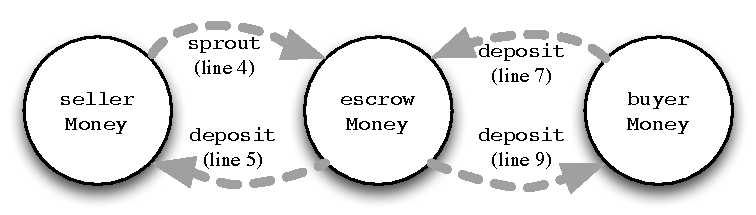
\includegraphics[scale=0.8]{mutual-trust-landscape.pdf}
  \vspace*{-4mm}
  \caption{Establishing Mutual Trust. Dashed arrows show purse validation.}
  \label{fig:mutual-trust}
\end{figure}
%
\noindent (Figure~\ref{fig:mutual-trust} illustrates the trust
relationships.)
If any of these
\prg{deposit} request fail, we abort.
% Lines~13--19 do
Afterwards we do exactly the same, but for goods purses rather than
money purses.  Finally, % lines~21--31
we carry out the escrow exchange
itself, in exactly the same manner as lines~8--29 of the first % escrow
implementation
in Figure~\ref{fig:DealV1}.


\paraC{Specifying the Mutual Trust Escrow}
\label{sec:VaildEscrow}


\begin{figure*}[hbt]
\begin{lstlisting}[escapechar=@]
specification ValidEscrow {
   fields sellerMoney, sellerGoods, buyerMoney, buyerGoods
   fields price, amt   // $\mathbb{N}$

 policy Pol_deal
  price,amt$\in \mathbb{N}$ $\wedge$ price,amt>0
      @\textbf{  \{  this.deal( \ ) \} }@
  res $\wedge$ BadPPrs=$\emptyset$  $\rightarrow$ (      //   1$^{st}$ case:
    CanTrade(buyerMoney,sellerMoney) $\wedge$
    CanTrade(buyerGoods,sellerGoods) $\wedge$
    buyerMoney.balance=buyerMoney.balance$\pre$-price $\wedge$
    sellerMoney.balance=sellerMoney.balance$\pre$+price$\wedge$
    buyerGoods.balance=buyerGoods.balance$\pre$+amt $\wedge$
    sellerGoods.balance=sellerGoods.balance$\pre$-amt $\wedge$
    $\forall$p:$\pre$OthrPrs. p.balance=p.balance.$\pre$  $\wedge$
    $\forall$o:$\pre$Object,p:$\pre$GoodPrs.
         ($\MayAccess$(o,p) $\rightarrow \MayAccess$(o,p)$\pre$) )
  $\wedge$
  $\neg$res $\wedge$ BadPPrs=$\emptyset$   $\rightarrow$ (   //   2$^{nd}$ case:
    $\neg$( CanTrade(buyerMoney,sellerMoney) $\wedge$
         CanTrade(buyerGoods,sellerGoods) $\wedge$
         buyerMoney.balance$\pre  \geq$ price $\wedge$
         sellerGoods.balance$\pre \geq$ amt ) $\wedge$
    $\forall$p:$\pre$GoodPrs. p.balance=p.balance.$\pre$   $\wedge$
    $\forall$o:$\pre$Object,p:$\pre$GoodPrs.
          ($\MayAccess$(o,p) $\rightarrow \MayAccess$(o,p)$\pre$)   )
  $\wedge$
  $\neg$res $\wedge$ BadPPrs$\neq$$\emptyset$  $\rightarrow$  (  //   3$^{rd}$ case:
    $\forall$p:$\pre$GoodPrs. (p.balance=p.balance.$\pre$ $\vee$
           $\exists$ bp$\in$BadPPrs$\pre.\, \MayAccess$(bp,p)$\pre$)  $\wedge$
    $\forall$o:$\pre$Object,p:$\pre$GoodPrs.( $\MayAccess$(o,p) $\rightarrow$
         ($\MayAccess$(o,p)$\pre$ $\vee \exists$b$\in$BadPPrs$\pre$.$\MayAccess$(b,p)$\pre$)) )
  $\wedge$
  res $\wedge$ BadPPrs$\neq\emptyset$   $\rightarrow$  (    //   4$^{th}$ case:
    buyerMoney$\obeys$ValidPurse $\longleftrightarrow$ sellerMoney$\obeys$ValidPurse  $\wedge$
    buyerGoods$\obeys$ValidPurse $\longleftrightarrow$ sellerGoods$\obeys$ValidPurse  $\wedge$
    $\forall$p:$\pre$OthrPrs. (p.balance=p.balance.$\pre$ $\vee$
        $\exists$bp$\in$ BadPPrs$\pre.\, \MayAccess$(bp,p)$\pre$)  $\wedge$
    $\forall$o:$\pre$Object,p:$\pre$GoodPrs. ($\MayAccess$(o,p)$\rightarrow$
       ($\MayAccess$(o,p)$\pre$$\vee \exists$b$\in$BadPPrs$\pre$.$\MayAccess$(b,p)$\pre$)) )
}
\end{lstlisting}
\vspace*{-7mm}
\caption{\prg{ValidEscrow} specification}
\label{fig:ValidEscrow}
\end{figure*}


%\forget{
%% SD made a shorter version
%\begin{figure*}[hbt]
%\begin{lstlisting}[escapechar=@]
%specification ValidEscrow {
%   fields sellerMoney, sellerGoods, buyerMoney, buyerGoods
%   fields price, amt   // $\mathbb{N}$
%
% policy Pol_deal_1    //   1$^{st}$ case:
%   price,amt$\in \mathbb{N}$ $\wedge$ price,amt>0
%      @\textbf{  \{  this.deal( \ ) \} }@
%    res $\wedge$ BadPPrs=$\emptyset$  $\rightarrow$ (
%      // FUNCTIONAL SPECIFICATION
%     CanTrade(buyerMoney,sellerMoney) $\wedge$                            CanTrade(buyerGoods,sellerGoods) $\wedge$
%      buyerMoney.balance=buyerMoney.balance$\pre$-price $\wedge$              sellerMoney.balance=sellerMoney.balance$\pre$+price$\wedge$
%      buyerGoods.balance=buyerGoods.balance$\pre$+amt $\wedge$                sellerGoods.balance=sellerGoods.balance$\pre$-amt $\wedge$
%      // RISK
%      $\forall$p:$\pre$OthrPrs. p.balance=p.balance.$\pre$  $\wedge$
%      $\forall$o:$\pre$Object,p:$\pre$GoodPrs.                                     $\MayAccess$(o,p) $\rightarrow \MayAccess$(o,p)$\pre$)
%
% policy Pol_deal_2    //   2$^{nd}$ case:
%    price,amt$\in \mathbb{N}$ $\wedge$ price,amt>0
%       @\textbf{  \{  this.deal( \ ) \} }@
%    $\neg$res $\wedge$ BadPPrs=$\emptyset$  $\rightarrow$ (
%       // FUNCTIONAL SPECIFICATION
%       $\neg$( CanTrade(buyerMoney,sellerMoney) $\wedge$                          CanTrade(buyerGoods,sellerGoods) $\wedge$
%            buyerMoney.balance$\pre  \geq$ price $\wedge$                            sellerGoods.balance$\pre \geq$ amt ) $\wedge$
%      // RISK
%      $\forall$p:$\pre$GoodPrs. p.balance=p.balance.$\pre$   $\wedge$
%      $\forall$o:$\pre$Object,p:$\pre$GoodPrs.                                        $\MayAccess$(o,p) $\rightarrow \MayAccess$(o,p)$\pre$  )
%\end{lstlisting}
%\vspace*{-7mm}
%\caption{\prg{ValidEscrow} specification}
%\label{fig:ValidEscrow}
%\end{figure*}
%%
%\addtocounter{figure}{-1}
%%
%\begin{figure*}[htb]
%\begin{lstlisting}[escapechar=@,firstnumber=38]
% policy Pol_deal_3    //   3$^{rd}$ case:
%    price,amt$\in \mathbb{N}$ $\wedge$ price,amt>0
%       @\textbf{  \{  this.deal( \ ) \} }@
%    $\neg$res $\wedge$ BadPPrs$\neq$$\emptyset$  $\rightarrow$  (
%       //RISK
%       $\forall$p:$\pre$GoodPrs. ( p.balance=p.balance.$\pre$ $\vee$                   $\exists$ bp$\in$BadPPrs$\pre.\, \MayAccess$(bp,p)$\pre$ $\wedge$
%       $\forall$o:$\pre$Object,p:$\pre$GoodPrs.$\MayAccess$(o,p)$\rightarrow$                    ($\MayAccess$(o,p)$\pre$$\vee \exists$b$\in$BadPPrs$\pre$.$\MayAccess$(b,p)$\pre$))
%
%
% policy Pol_deal_4    //   4$^{th}$ case:
%    price,amt$\in \mathbb{N}$ $\wedge$ price,amt>0
%       @\textbf{  \{  this.deal( \ ) \} }@
%    res $\wedge$ BadPPrs$\neq\emptyset$    $\rightarrow$  (
%      // TRUST
%      buyerMoney$\obeys$\tobym{ValidPurse} $\longleftrightarrow$ sellerMoney$\obeys$\tobym{ValidPurse}  $\wedge$
%      buyerGoods$\obeys$\tobym{ValidPurse} $\longleftrightarrow$ sellerGoods$\obeys$\tobym{ValidPurse}  $\wedge$
%      //RISK
%      $\forall$p:$\pre$OthrPrs. ( p.balance=p.balance.$\pre$ $\vee$                                  $\exists$ bp$\in$ BadPPrs$\pre.\, \MayAccess$(bp,p)$\pre\  )$   $\wedge$
%       $\forall$o:$\pre$Object,p:$\pre$GoodPrs.$\MayAccess$(o,p)$\rightarrow$                   ($\MayAccess$(o,p)$\pre$$\vee \exists$b$\in$BadPPrs$\pre$.$\MayAccess$(b,p)$\pre$))
%}
%\end{lstlisting}
%\vspace*{-7mm}
%\caption{\prg{ValidEscrow} specification (contd.)}
%\end{figure*}
%}


Figure~\ref{fig:ValidEscrow}~shows a specification for the revised
escrow deal method from Figure~\ref{fig:DealV2}.  This specification
uses conditional and hypothetical reasoning to
distinguish four cases, based on the value of the result and
the trustworthiness of the participants.
%
We use these auxiliary definitions:
%
\begin{lstlisting}[numbers=none,frame=none,rulecolor=\color{white}]
GoodPrs$=\{$ p | p $\obeys\PRE$ ValidPurse $\}$
PPrs$=\{$ sellerMoney, sellerGoods, buyerMoney, buyerGoods $\}$
OthrPrs$=$GoodPrs $\setminus$ PPrs
BadPPrs$=$PPrs $\setminus$ GoodPrs
\end{lstlisting}
%
\vspace*{-3ex}
%
\noindent The set \lstinline{PPrs} contains the four \emph{participant purses}
passed as arguments.
\lstinline{BadPPrs} contains the untrustworthy participant purses.
\lstinline{GoodPrs} are all trustworthy purses in the system
that do conform to the \lstinline{ValidPurse} specification, and
\prg{OthrPrs} are the trustworthy purses that do
\textit{not} participate in this particular deal.
We can now discuss the four cases of the policy:

% \begin{description}

\textbf{1$^{st}$ case:} The result is \prg{true} and all participant
  purses are trustworthy. Then, the goods and money purses
  can trade with each other, and there was sufficient
  money in the buyer's purse and sufficient goods in the sellers purse.
  In this case, everything is fine, so the transfer can proceed:
  \prg{price} will have been transferred from the buyer's to the
  seller's money purse, and \prg{amt} will have been transferred from
  the seller's to the buyer's goods purse.
  No risk arises:
  no other
  purses' balance will change (whether passed in to
  the method or not).


\textbf{2$^{nd}$ case:} The result is \prg{false} and all
participant purses are trustworthy. Then
one or more of  the functional correctness conditions are
  not satisfied: purses' were unable to trade with each other, or input
  purses did not have sufficient balance. Again, no risk arises
  to any purses.


\textbf{3$^{rd}$ case:} The result is \prg{false} and some participant purse is untrustworthy.
  In this case, no   trustworthy purses' balances have been changed --- unless
  they were already accessible by an untrustworthy purse passed in to
  the method.

\textbf{4$^{th}$ case:}  The result is \prg{true}  and some participant
  purse is untrustworthy --- actually at least two
  matching participant purses are untrustworthy.
  %% Do not change the above. The previous change was wrong.
  That is, a pair of matching purses
  have co{\"o}perated to
  suborn the escrow \textit{and we cannot tell}.
 Therefore, either both money purses are untrustworthy,
 (as per line 35),  % \\
 % NOT either - or; they can both be
% \begin{lstlisting}
% buyerMoney$\obeys$\tobym{ValidPurse} $\longleftrightarrow$ sellerMoney$\obeys$\tobym{ValidPurse}
% \end{lstlisting}
or both goods purses are untrustworthy,
 (as per line 36),
%\begin{center}
% $ ~ $ \SP\SP \lstinline+buyerMoney$\obeys$\tobym{ValidPurse}+ $\longleftrightarrow$\\
% $ ~ $ \SP\SP \lstinline+sellerMoney$\obeys$\tobym{ValidPurse}+\\
%\end{center}
%
%
%
% \noindent or both goods purses are untrustworthy (line )
% :\\
%
%
%\begin{center}
% $ ~ $ \SP\SP \lstinline+buyerGoods$\obeys$\tobym{ValidPurse} $\longleftrightarrow$+\\
% $ ~ $ \SP\SP \lstinline+sellerGoods$\obeys$\tobym{ValidPurse}+ \\
%\end{center}
%
% \begin{lstlisting}
% buyerGoods$\obeys$\tobym{ValidPurse} $\longleftrightarrow$ sellerGoods$\obeys$\tobym{ValidPurse}
% \end{lstlisting}
%
%\noindent
or all four are bad. % As we've argued above, in this
% circumstance an implementation cannot tell whether the purses are good
% or not, so we permit the method to return \prg{true}.
%
The risk is that an uninvolved trustworthy purse's balance can be
changed if it was previously accessible from a bad purse.
%
% \end{description}
%
%
%
The first and second cases correspond to a traditional
specification, because traditional specifications assume all objects
are trustworthy.  The third and fourth cases arise precisely because
we are explicitly modelling the trust and risk involved in an open
system.

\paragraph{Discussion} The 3$^{rd}$  and 4$^{th}$ case represent  more
of a risk than we would like: ideally (as
  in the 2$^{nd}$ case) we'd hope nothing should have changed. But an
  escrow method cannot undo a system that is already suborned --- if
  one of the participant purses is already benefiting from a security
  breach, passing that purse in to this method gives it an opportunity
  to exercise that breach.  On the other hand, the risk is contained:
  this method cannot make things worse.
%

The
 4$^{th}$ case does not prevent trustworthy participant purses from
 being modified, to cater e.g., for the possibility that the two money
 purses are  trustworthy, while the two goods purses are not, in which
 case  the money transaction will take place as expected,  while all
 bets are off about the goods transaction.
 We can give the stronger guarantee for the 3$^{rd}$ case, because by
 the time the escrow starts making non-$0$ transactions \jnCUT{(line
   24 onwards in Fig.\  7)} it has established that the purses in each
 pair are both either trustworthy or both not.

Most importantly (perhaps surprisingly)
the return value of the method, \prg{res}, does {\em not} indicate
whether the participants were trustworthy or not. A \prg{true}
result may be returned in the 1$^{st}$ case (all purses trustworthy)
as well as the 4$^{th}$ (some purses are untrustworthy).  The
return value indicates {\em only} whether the escrow attempted to complete the
transaction (returning \prg{true}) or abort (returning
\prg{false}). This came
 as a surprise to us (and to the escrow's designers \cite{miller-esop2013}.)
As with much of our reasoning around trust,
this leads to yet more conditional reasoning, which must be
interpreted hypothetically.

Nevertheless, the return value does communicate a valuable guarantee to an honest
participant,   whose money and goods purses are both
trustworthy:  If \prg{deal} returns \prg{true}, then the exchange has taken
place. Furthermore if it returns \prg{false}, the exchange has not taken
place and with \textit{no more} risk to the honest purses than existed before the call.
%
%
%
% \footnoteC{SD I dropped the following as the point is that in case 4,
%   the escrow does NOT detect untrustworthiness, but perhaps you can
%   turn it to something else and useful.
% \jn{again, trying to distinguish between cases 3 and 4}
%
% Note also that the 3rd and 4th case overlap: the specification is
% nondeterministic where untrustworthy purses are involved.  If an
% implementation somehow detects the untrustworthiness and aborts the
% swap, it may return \prg{false} providing that the participating
% purses' balances have not be changed (modulo pre{\"e}xisting access
% from bad purses). Alternatively, the method may return \prg{true} and
% make no guarantees about the balances of any of the
% participating purses.}
%
The \prg{ValidEscrow} specification also gives a guarantee to other
purse objects even if they did not participate in the deal:
dishonest purses can only change
other purses' balances if they had prior access to those other purses.


\section{A Formal Model of Trust and Risk}
\label{section:formal}
 
In this section we provide an overview of our core programming
language, \LangOO, our specification language, \Chainmail, and our
Hoare logic. \kjx{The Hoare logic uses \textit{four-tuples} because it
  includes an invariant that must be preserved during the execution of
  a statement as well as a postcondition established afterwards.}
\kjx{We also outline a key step required to prove} that
\prg{deal\_version2} meets the \prg{ValidEscrow} specification:
\kjx{we prove that two purses can establish mutual trust, and formally delineate
the risk.}  Many
details are relegated to our technical report \cite{appendix}; here we
adopt its numbering for definitions.




\subsection{\LangOO}

We define a small object oriented language, \LangOO\ 
(Featherweight Object Capability Language, not to be confused
with FOCAL \cite{FOCAL-69}). \LangOO\ 
 supports classes, fields and methods.
(Figures~\ref{fig:DealV1} and~\ref{fig:DealV2} are effectively examples of \LangOO.)
%
\LangOO\ is  memory-safe: it does not allow
addresses to be forged, or non-existent methods or fields to be
called, read or written.   \LangOO\ is dynamically typed: it does not check
that the arguments to a method call or a field write are of the
appropriate type either statically or dynamically: similar to 
JavaScript, Grace, E, and Dart's unchecked mode.
 

% \LangOO\  supports
Modules, $M$,  are  mappings from class
identifiers to \LangOO\ class definitions, and from predicate identifiers to \Chainmail\ assertions as described in section \ref{sect:Chainmail}.
The  linking operator $*$ combines these definitions, provided that 
the modules' mappings have separate domains, and performs no other checks. 
This reflects the open world setting,
where objects of different provenance interoperate without a central
authority.
For example, taking $M_{p}$ as a module implementing purses, and $M_e$
as another module implementing the escrow,
$M_{p}*M_e$ is defined but $M_{e}*M_e$ is not.

\LangOO\  enforces a weak form of privacy for fields; % are \prg{private}; 
only the receiver may modify these fields,  and anybody may read them.
% SD what it said before is wrong, and did not come from Appendix :-(
%THIS IS STILL PROBABLY WRONG!

The operational semantics of  \LangOO\ takes a module $\M$  
and a runtime state $\sigma = \syntax{frame} \times \syntax{heap}$ 
and maps statements onto a new 
state $\sigma'$.
% This is not needed for the main paper
% and right hand sides of assignments (\ie paths, values, and method calls) to a value and new state and a value. 
%The
% operational semantics has the following shape: 

\vspaceSD

\setcounter{definition}{5}
\begin{definition}[Shape of Execution]

\begin{tabular}{lcl}
 ${\rewriteLong {}}\s$ &  :  &    \syntax{Module}  $\times$  \syntax{state}  $\times$   {\syntax{Stmts}}
  \ \  $\longrightarrow $ \ \     {\syntax{state}}
%\\
% ${\rewriteLong {}}\s$ &  :  &    \syntax{Module}  $\times$  \syntax{state}  $\times$   {{\syntax{Rhs}}}
%  \ \  $\longrightarrow $ \ \     \syntax{heap} $\times$ \syntax{val}  
\end{tabular}
\end{definition}




 
\paragraph{Arising and Reachable Configurations}  

Policies need to be satisfied in all {\em configurations} (pairs of states and statements) which may
arise during execution of the program. For example, if a program contains a class which has field which is not exported, and
where this field is initialized to $0$ by the constructor, and incremented by $3$ in all method calls, then in the arising configurations the
value of this field is guaranteed to be a multiple of $3$. Thus, through the concept of arising configurations we can 
ignore configurations which are guarantee not to arise.

To define arising configurations we need the concept of initial configuration, and reachability. 
 A configuration is
\emph{reachable} from some starting configuration if it is reached
during the evaluation of the starting configuration after any number
of steps.     We define
the function 
\mbox{$\Reach:\syntax{Module} \times \syntax{state} \times \syntax{Stmts} 
\longrightarrow \mathcal{P}(\syntax{state} \times \syntax{Stmts})$}
by cases on the structure of
the statements. Note that  $\Reach(\M, \sigma, \stmts) $ is defined, 
even when the execution should diverge. This is important, because it allows us to give meaning to capability policies without requiring termination. 


\noindent We then define $\Arising(\M)$ as the set of runtime configurations
which may be reached during execution of some initial context
($\sigma_0$,$\code_0$).

\setcounter{definition}{6}
\begin{definition}[Arising and Initial configurations] 
$ ~ $

$\begin{array}{lcl}
\SP {\mathcal{I}nit} & \ : \ & {\syntax{Module}} \   \longrightarrow\  \mathcal{P}( {\syntax{state} \times \syntax{Stmt}}  )
\\
 \Arising & : &  {\syntax{Module}}    \longrightarrow \mathcal{P}( {\syntax{state}} \times \syntax{Stmts}  )
\end{array}$

$\begin{array}{ll}
 {\mathcal{I}nit}(\M)   =  &  \{ \ (\ \sigma_0, \kw{new}\ \clss{}.\prg{m}\lp\kw{new}\  \clss{'} \rp) \ |    \ \clss{},\clss{'}\in dom( \M),\\
 & \ \ \ 
   \mbox{where}\  \sigma_0\ =\ ( (\iota_0,\kw{null}),\chi_0),    \mbox{and}\   \chi_0(\iota)=(\prg{Object}, \emptyset)\  \}
 \\
 \Arising(\M)    =   & \    \bigcup_{ (\sigma,\code{})\in  \mathcal{I}nit (\M)}  \Reach(\M, \sigma, \code{})
\end{array}$
\end{definition}




\subsection{\Chainmail}
\label{sect:Chainmail}

\Chainmail\ is a specification language where a specification is
a conjunction of a set of named policies.
(Figures~\ref{fig:ValidPurse} and~\ref{fig:ValidEscrow} are examples of
\Chainmail\ specifications.)

\Chainmail\ policies are based on one-state assertions ($\A$) and two-state assertions ($\B$).  To express the state in which an expression
is evaluated, we annotate it with a subscript. For example, $x>1$ is a one-state, and 
$ x\pre - x\post = 1$ is a two-state assertion. Validity of an assertion is defined in the usual manner, \eg 
in a state $\sigma$ with  $\sigma(x)=4$ we have   $M,\sigma \models x>1$. If we also have $\sigma'(x)=3$,
then we obtain    $\M,\sigma,\sigma' \models x\pre - x\post =
1$.  \Chainmail\ specifications may also express ghost information,
which is not stored explicitly in the state $\sigma$ but can be
deduced from it --- e.g.\ the length of a null-terminated string.



Policies can have one of the three following forms:  
1) invariants of the form $\A$, which   require that $\A$ holds at all visible states of a 
program; or  
2)\  $\A\, \lb \, \prg{code}\, \rb\, \B$, which require that execution of \prg{code} in any state satisfying $\A$ will lead to a state
satisfying $\B$ wrt the original state
 or  
 3)\ $\A\, \lb \,  {\prg{any\_code}}\, \rb \, \B$ which requires that execution of {\em any} 
 code in a state satisfying $\A$ will lead to a state satisfying $\B$ wrt the original state.

\vspaceSD

\setcounter{definition}{11}
\begin{definition}[Policies]
 $ ~ $ \\
 $
\begin{array}{lclcl}
Policy & \BBC & \ \A \ | \  \A \ \{ \prg{code} \}\  \B \ | \ \  \A \ \{ \prg{any\_code} \}\ \B
\\
PolSpec & \  \BBC  & \  \prg{specification}\ S \, \lb\, Policy^*\, \rb
\end{array}
$
\end{definition}


One-state assertions include assertions about  expressions (such as $\leq$, $>$ \etc) and four additional
assertions: $\syntax{\sExpr}\obeys\syntax{SpecId}$ to model trust,
i.e.\ that an object confirms to a specification; and $\MayAccess$ and
$\MayAffect$ to model risk, i.e.\ whether one object may access
another, or alter a property.  These are {\em hypothetical}, in that
they talk about the potential effects or behaviour of code: we cannot
somehow evaluate their truth-value when executing the program.  The
fourth assertion $\syntax{\sExpr}\kw{:}\syntax{ClassId}$ 
simply tests class membership. 
 
 
Validity of one-state assertions is expressed through the judgment
$\M,\sigma \models \A$.  The key case is that some expression obeys a
specification if it satisfies that specification's policies in all
reachable configurations arising from the module.

 

\vspace*{1mm}\noindent\textbf{(from Definition 13)}:

\begin{itemize}
  \item
 $\M,\sigma  \models  \syntax{\sE}\kw{:}\prg{C}$ iff  $\sigma(\interp{ \syntax{\sE}}{\M,\sigma})\downarrow_1 = \prg{C}$.
 
 \item 
$\M,\sigma  \models \MayAffect \lp\syntax{\sE},\syntax{\sE'}\rp$ iff  
% there exist fields  $\prg{f}_1$,... $\prg{f}_n$,  
there exist  method \prg{m}, arguments $\bar{\prg{a}}$, state $\sigma'$, identifier \prg{z}, such that
    $ \M, \sigma[\prg{z}\mapsto \interp {\syntax{\sE}} {\M,\sigma}], \syntax{z}\prg{.m}(\bar{\prg{a}}) \leadsto   \chi'$, and   $\interp {\syntax{\sE'}} {\M,\sigma} \neq  \interp {\syntax{\toby{\sE'}}} {\M,\sigma\downarrow_1,\chi'}    $.
\item
$\Prog{},\sigma \models { \MayAccess}(\prg{\sE},\prg{\sE'})$   \ iff \  there exist  fields $\bar{\prg{f}}$, % $\prg{f}_1$,... $\prg{f}_n$, 
  such that
     %  $\interp{\prg{z}.\prg{f}_1...\prg{f}_n}{\M,\sigma[\prg{z}\mapsto \interp {\syntax{\sE}} {\M,\sigma}]}= \interp {\prg{\sE'} }{\M,\sigma}$.
     $\interp{\prg{z}.\ensuremath{\bar{\prg{f}}}}{\M,\sigma[\prg{z}\mapsto \interp {\syntax{\sE}} {\M,\sigma}]}= \interp {\prg{\sE'} }{\M,\sigma}$
  \item
$\M, \sigma  \models \sE \obeys \PolSpecId   $ \  iff  \\
\SP  $\ \ \   \forall\, (\sigma,\code)\!\in\!\Arising(M).\   \forall  i\!\!\in\! \!\{1..n\}. \ \forall\,\sigma',\code'.$  \\
\SP  $\ \ \    (\sigma',\code')\! \in \Reach(M,\sigma,\code)  \longrightarrow    M, \sigma'[z\mapsto\interp{e}{\sigma}]  \models \Policy_i[ z / {\kw{this}}]$ \\
where $z$ is a fresh variable in $\sigma'$, and where
 we assume that $\PolSpecId$ was defined as \ \  %  that   \PolSpecId was introduced by\\
$ \ \prg{specification}\ \PolSpecId\  \{\ \Policy_1, ... \Policy_n\ \}$. \\
\end{itemize}
% \end{definition}

Two-state assertions allow us to compare properties of two different
states. Validity of two-state assertions $\M,\sigma,\sigma' \models \B$
is defined similarly to one-state assertions, using cases.
%
We can now define adherence to policy, $\M,\sigma \models_{pol}  \Policy$:
%    which
% ensures that the requirements of $\Policy$ are satisfied in any context arising from $\M$.

\vspaceSD
\setcounter{definition}{14}
\begin{definition}[Adherence to Policies] ~ ~ % \\
% $ $ \\

\begin{itemize}
\item
$\M,\sigma  \models_{pol} \A$   \  iff \ 
$\M, \sigma \models \A$
\item
$\M,\sigma    \models_{pol} \A\, \{ \prg{code} \}\, \B$ \  iff \\ 
 $ ~ $ \hspace{.2in} 
 $(\ \M, \sigma \models \A\ \ \wedge\  \M, \sigma, \prg{code}  \leadsto \sigma' $ %  \\
 %  $ ~ $   \hspace{.6in}  
 $ \ \ \  \longrightarrow $ 
%  \\  $ ~ $   \hspace{.2in}  
$  \ \ \ \M, \sigma, \sigma' \models \B\ \ )$
\item
{$\M, \sigma \models_{pol} \A \ \{ \prg{any\_code} \}\ B$\ iff} \\
 $ ~ $ \hspace{.2in}  $ \forall \prg{code}.\ (\  (\sigma,\prg{code} )\in \Arising(\M)\ \wedge\  \M, \sigma \models \A\  \wedge\  \M, \sigma, \prg{code}  \leadsto  \sigma' $ \\
  $ ~ $   \hspace{.6in}  $ \ \ \  \longrightarrow $
  % \\   $ ~ $   \hspace{.2in}  $ 
   $\ \ \ \M, \sigma, \sigma' \models \B\ \ )$
\end{itemize}
\end{definition}

% SD removed it, ad not central and moved the for all modules to later on
%\setcounter{definition}{14}
%\begin{definition}[Strong Adherence to Policies] ~ ~ % \\
%% $ $ \\
%
%\noindent $\M   \models_{pol} Policy$   \  iff \ \\
%\SP $\forall \M', \sigma, \code. \ 
%(\ (\sigma,\code)\in \Arising(\M'*\M)\ \longrightarrow \M'*\M, \sigma \, \models Policy\ )$
%\end{definition}


\subsection{Hoare Logic}

The Hoare logic allows us to prove adherence to policies. In order to
reflect that the code to be verified is executed in an open system,
and that it calls code whose specification and trustworthiness is
unknown to the code being verified, we use Hoare four-tuples rather
than Hoare triples, so that not only do they guarantee a postcondition
holds {\em after} execution of the code, but also guarantee that
\kjx{an invariant} is preserved {\em during} execution of the code.
\kjx{These invariants are critical to modelling risk, as they let us 
talk about the absence of temporary but unwanted effects caused on
objects during execution.}% e.g.\ reasoning  that valid purses
%always correctly protect their balances.}


\kjx{A Hoare four-tuple  is either \mbox{\HoareExpl{\A}
  {\prg{stms}} {\M} {\A'} {\B}} (executing 
\prg{stms} in any state satisfying $\A$~will lead to a state which
satisfies $\A'$) or \mbox{\HoareExpl{\A} {\prg{stms}} {\M} {\B'} {\B}}
(executing \prg{stms} in any state satisfying
$\A$~will lead to a state where the relation of the old and
new state is described by $\B'$).}  \kjx{Critically,} both promise that the relation between
the initial state, and {\em any} of the   intermediate states reached by
execution of \prg{stms}, will \kjx{maintain the invariant} $\B$.
The execution of \prg{stmts}  may call methods defined in \M, and the
predicates appearing in $\A$, $\A'$, $\B'$, and $\B$, may use  predicates
  defined in \M. 
When \M\ is implicit from the context,
we use the shorthand
\Hoare{\A} {\prg{stms}}  {\A'} {\B}. 


In order to model open systems, we require that after linking {\em any}
module with the module at hand, the policy will be satisfied. As
stated in \cite{JamesMorris}, \textit{``A programmer should be able to prove
that his programs have various properties and do not malfunction,
solely on the basis of what he can see from his private bailiwick.''}

% SD removed as not cnetral to our argument
% We introduce {\em logical variables} into our assertions. We assume that
%these have the form \lvar, \lvar', and that they come from a separate domain. We also
% assume that there exists a function \Lvars, which returns all the
% logical variables within an assertion. For example
% $\Lvars(\prg{p1.balance}=\lvar ) =\{\,\lvar\,\}$. Taking account of
% logical variables we can define the validity of tuples formally:
 
\vspace{-.05in}
\begin{definition}[Validity of Hoare Four-Tuples]\label{defn:validity}

\noindent
%  \begin{itemize}
%  \item
%$M  \models \HoareImpl{\A} {\prg{stms}0.5} {\A'} {\B}  $ \ \ \  iff\\
%\SP $ \Lvars(\A)=\Lvars(\A')=\{\, \overline{\lvar}\, \}\ \wedge \ \forall \M',\sigma, \overline{\val}.$\\
%\SP\SP $ (\sigma,\_)\in \Arising(\M*\M')$\\
%\SP\SP $ \wedge\ \M*\M',  \sigma{[\overline{\lvar}\mapsto\overline{\val}]} \models \A$\\
%\SP\SP $ \wedge\  \M\!*\!\M', \sigma, \prg{stms}  \leadsto \prg{res}, \sigma'$\\
%\SP\SP\SP \ \ \ $\longrightarrow$ \ \ \ \\
%\SP\SP   $ \M\!*\!\M'\!, \sigma'{[\overline{\lvar}\mapsto\overline{\val}]} \models \A' $\\
%\SP\SP    $\wedge$ \\
%\SP\SP  $\forall {\sigma''}\!\in\!\Reach(M,\sigma,\stmts).\ \M\!*\!\M', \sigma, {\sigma''} \models \B   $
%  \item
$M  \models  \HoareImpl{\A} {\prg{stms}} {\B'} {\B}  $ \ \ \  iff \ \ 
  $\forall \M',\sigma$.\\
\SP $ (\sigma,\_)\in \Arising(\M*\M')\  \ \wedge  \ \ \M*\M',  \sigma \models \A \  \ \wedge \ \   \  \M\!*\!\M', \sigma, \prg{stms}  \leadsto \prg{res}, \sigma'$\\
\SP\SP\SP\SP\SP\SP\SP\SP\SP\SP\SP \ \ \ $\longrightarrow$ \ \ \ \\
\SP $M\!*\!\M'\!, \sigma, \sigma' \models \B' \ \ \ \wedge \ \ \forall {\sigma''}\!\in\!\Reach(M,\sigma,\stmts).\ \M\!*\!\M', \sigma, {\sigma''} \models \B $
% \end{itemize}
\end{definition}


\renewcommand{\true}{true}

\begin{figure*} 
$\begin{array}{l}
 \begin{array}{lcl}
      \inferenceruleNP {varAsg} {
} {
         \Hoare {\true}
      {  \prg{v} \kw{:=} \prg{a} } { \prg{v}=\prg{a}\pre }  {\true}
}
& \SP\SP  &
\inferenceruleN{fieldAsg} {
 
}{
     \Hoare
     {\true}
      { \kw{this.}\prg{f}  \kw{:=} \prg{a} }
      { \kw{this.}\prg{f}   = \prg{a}\pre}
       {\true}
}
\end{array}
\\ \\
  \inferenceruleNNP {meth-call-1} {
    { \M(S) \,= \,  \kw{spec}\ S\  \lb\  \overline{Policy}, \A \,\lb \, \prg{this.m(par)}\, \rb\, \B, \overline{Policy'}\  \rb}
% \SP\SP \SP\SP\SP
  %  \B''[\prg{x}/\prg{this},\prg{y}/\prg{par}] = \B'''
    } {
    \Hoare{\prg{x}\obeys S\wedge  \A[\prg{x}/\prg{this},\prg{y}/\prg{par}]} {\prg{v} \, \kw{:=}\, \prg{x.m(y)}} {\B[\prg{x}/\prg{this},\prg{y}/\prg{par},\prg{v}/\prg{res}]}   {{\true}} % {\B'''}
  }
  \\
  \\
   \inferenceruleNNP {meth-call-2} {
         \B \equiv \forall \prg{z}:\pre \Obj.\ \MayAccess({\prg{v},\prg{z}}) \rightarrow  
    (\, \MayAccess\pre(\prg{x},\prg{z})\, \vee \, \MayAccess\pre(\prg{y},\prg{z})\, )\\
   \B' \equiv   \forall \prg{z},\prg{u}:\pre \Obj. \ ( \ \MayAccess({\prg{u},\prg{z}}) \rightarrow \\
       $ ~ $ \hspace{1.3in}  ( \MayAccess\pre(\prg{u},\prg{z}) \ \ \ \vee  \\
                 $ ~ $ \hspace{1.7in}(\  (\MayAccess\pre({\prg{x},\prg{z}})\vee \MayAccess\pre({\prg{y},\prg{z}}) )\ \wedge \\
                 $ ~ $ \hspace{1.8in}  (\MayAccess\pre({\prg{x},\prg{u}})\vee \MayAccess\pre({\prg{y},\prg{u}}) ) \ ) \ ) \ \  )  } {
    \Hoare{\true} {\prg{v} \, \kw{:=}\, \prg{x.m(y)}} {\B}
           { \B'  }
}
\\ \\
   \inferenceruleNNP {frame-methCall} {
          \Hoare{\A}   {v:=\prg{x.m(y)}} {{\true}}  {\B} \\
B \equiv \forall \prg{z}. (\ \MayAffect(\prg{z},\A')  \rightarrow \B'({\prg{z}})\ )\ \ \wedge 
          \\
% trick for layout
		\SP\SP  \ 
		{\forall \prg{z}.(\ (\MayAccess(\prg{x},\prg{z}) \vee \MayAccess(\prg{y},\prg{z})
           \vee \New(\prg{z}) \ )%(\prg{z}:\prg{Object}\wedge \neg ( \prg{z}:\pre\prg{Object}) ) \ )
           \ \rightarrow\  \neg \B'(\prg{z})\ )}
}
{
          \Hoare{{\A\wedge\A'}} {\prg{v:=x.m(y)}} {\A'} {{\true}}
}
\\ \\
\begin{array}{lcl}
 \inferenceruleB {\SP\SP\SP\SP\SP\SP\SP\SP\SP\SP}   {code-invar-1} {
            { \M( S) \equiv \  \kw{spec}\ S\  \lb\  \overline{Policy}, P, \overline{Policy'}\  \rb}
            \\
            \B \equiv {\forall \prg{x}.(\, \prg{x} \obeys S \rightarrow P[/\prg{x}/\prg{this}]\, )}
  }
     {
       \Hoare {{\true}} {\stmts} {{\true}} {\B}
      }
      & &
\inferenceruleB {\SP\SP\SP\SP\SP\SP\SP\SP\SP\SP}   {code-invar-2} {           ~ \\
     }{
    \Hoare  {e \obeys S}  {\stmts}    {\true}  {e\pre \obeys S}
      }

\end{array}
\\ \\
\begin{array}{lcccr}
  \inferenceruleNP{Cons-2} {  % NEW
          \Hoare{\A}{\stmts}{ \B}{\B''}   \\
           \sd{\A',\B' \rightarrow_\M \A,\_}   
     }
     {
       \Hoare{\A'}{\stmts}{\sd{\B'\!\rightarrow\!\B}}{\B''}
        }
        &\ \ &
\inferenceruleNP {Cons-3} 
{ 
  \Hoare{\A}{\stmts}{ \B}{\B'} %
  \\
 {{\A}, \B \rightarrow_\M \_,\A'}  
} {
   \Hoare{{\A}}{\stmts}{ \A'}{\B'}
   }
&    &
  \inferenceruleNP {Cons-4} { % was Cons-2 
          \Hoare{\A}{\stmts}{ \A'}{\B'}  
        \\
     {{\A},\A' \rightarrow_\M \B}  
     }
     {
       \Hoare{\A}{\stmts}{ \B}{{\B'}}
        }
 \end{array}
\\ \\
\inferenceruleNNP{sequence} {
        \Hoare{\A}{\stmtss_1}{\B_1}{\B'}  \ \SP        \Hoare{\A_2}{\stmtss_2}{ \B_2}{\B'}
        % \\
       \ \SP
         {\A,\B_1\rightarrow_\M \_,\A_2}    \ \SP  {\B_1,\B_2\rightarrow_\M \B}
        }
     {
       \Hoare{\A}{\stmtss_1; \, \stmtss_2}{ \B}{\B'}
        } 
\end{array} 
$
\caption{A selection of Hoare Logic rules; we assume that the module \M\ is globally given}
\label{fig:HoareLogic}
\end{figure*}

% \noindent
Figure \ref{fig:HoareLogic} shows a selection of our Hoare rules. It starts with two familiar Hoare Logic rules: In \ruleN{varAsg}  and \ruleN{fieldAsg}  the postconditions
use the previous value of the
right-hand-side, and thus  allow us to deduce, \eg: \\ % that\\
\SP \SP \Hoare {\kw{this}.f=21} {\kw{this}.f=2*\kw{this}.f} {\kw{this}.f=42}  {\true}.
\\
%\vspace{.1in}
%
\scd{\ruleN{meth-call-1} is also familiar, as it reasons over method calls under the assumption that the 
receiver   \obeys a specification $S$, and that the current state satisfies the precondition of 
\prg{m} as defined in $S$.}
% by making use of the \obeys assertion.

The remaining rules are more salient.

\ruleN{meth-call-2} expresses the basic axiom of object-capability
systems that ``only connectivity begets connectivity''~\cite{MillerPhD}.
\tobym{It promises in the postcondition that the result of the method call~\prg{v} 
cannot expose access to any object \prg{z} that wasn't
accessible initially to the method call's receiver~\prg{x} or argument~\prg{y}.
Additionally, it also promises that,
{\em during} execution of the method, accessibility does
not change, unless the participants (here \prg{z}  and \prg{u})
were accessible to the receiver and/or the argument {\em before}
the call. Note that this latter promise is made via the invariant (fourth)  rather than  the postcondition (third) part
of the Hoare-tuple. Note also that this rule is applicable {\em even if we know nothing} about the 
receiver of the call:}
\kjx{this rule and the invariants are critical to reasoning about risk.}

\ruleN{code-invar-1} allows reasoning under the hypothesis that
an object~$o$ \obeys its specification~$S$: in this case~$o$ can be trusted
to act in accordance with~$S$ always.


\ruleN{frame-methCall} also
expresses an axiom of object-capability languages, namely that
in order to cause some visible effect, one must have access to an object able
to perform the effect. Coupled with ``only connectivity begets connectivity'',
this implies that a method can cause some effect only if the caller has
(transitive) access to some object able to cause the effect (including
perhaps the callee).


The remaining rules each make use of the entailment judgement~$\rightarrow_M$,
which allows converting back and forth
between one-state and two-state
assertions and comes in number of flavours; the relevant ones are
defined as follows.

\setcounter{definition}{18}
\begin{definition}[Entailment]
\label{def:entail}
$ $ \\

\begin{enumerate} 
\item
\label{entailPQPP}
{
$\A, \B \rightarrow_\M \A',\A''$\ \  iff\ \\
$\forall \sigma, \sigma'. \ \sigma\models \A\ \wedge\  \sigma,\sigma' \models \B \ \ \longrightarrow\ \ \sigma \models \A' \ \wedge\  \sigma' \models \A''$}
\item
\label{entailPPQ}
{$\A, \A' \rightarrow_\M \B$}\ \  iff\ \\
{$\forall \sigma, \sigma'. \ \sigma\models \A\ \wedge\  \sigma' \models \A'\  \ \longrightarrow\ \  \sigma,\sigma' \models \B$}
\item
\label{entailQQQ}
{$\B, \B' \rightarrow_\M \B''$}\ \  iff\ \\
{$\forall \sigma, \sigma', \sigma''. \  \sigma,\sigma' \models \B\ \wedge\   \sigma',\sigma'' \models \B'\  \ \longrightarrow\ \  \sigma,\sigma'' \models \B''$}
\end{enumerate}
\end{definition}

The rules \ruleN{cons-3} and \ruleN{cons-4} make use of the entailment
judgement to allow converting between one- and two-state postconditions
during Hoare logic reasoning.
To reason across sequenced computations $\stmtss_1; \stmtss_2$,
the \ruleN{sequence} rule requires finding a one-state assertion~$\A_2$ 
that holds after $\stmtss_1$ and is the precondition of $\stmtss_2$. It uses
the entailment $\A, \B_1 \rightarrow_M \_,\A_2$ to require that
$\stmtss_1$'s execution guarantees $\A_2$, and the entailment
$B_1, B_2 \rightarrow_M B$ to require that the combined execution
of $\stmtss_1$ and $\stmtss_2$ guarantees the top-level postcondition~$B$.

 % \scd{Soundnss of the Hoare rules is stated below, and proven in \cite{appendix}}

\noindent

\setcounter{theorem}{2}
\begin{theorem}[Soundness of the Hoare Logic]

 For all modules \M, statements \prg{stms} and assertions $\A$, $\B$ and $\B'$ ,  
\\
$\SP\SP$ If \ \ $\HoareExpl {\A} {\prg{stms}}{\M}  {\B'} {\B}$, \   then\  $\M \models \HoareImpl {\A} {\prg{stms}} {\B'} {\B}$.  

\end{theorem}

\noindent
\scd{The theorem is proven in \cite{appendix}.}


\vspace{.05in}
\noindent 
\scd{In summary, we have four ''code agnostic'' rules ---
% SD I am happy if you find a better word than code-agnistiv, 
rules which 
are applicable regardless of the underlying code. Rules \tobym{\ruleN{frame-methCall} 
and \ruleN{meth-call-2}}  express  restrictions on the effects of a
method call.
\kjx{Normally such restrictions stem from the specification of the
  method being called, but here we can argue in the absence of any
  such specifications, allowing us to reason about risk even in open systems.}
Rules \ruleN{Code-Invar-1}  and \ruleN{Code-Invar-2} are applicable on {\em any} code, and allow us to
assume that an object which \obeys a specification $S$, satisfies all policies from $S$, and that the
object, once trusted, will always be {\kw {obeying}} $S$.}


\subsection{\kjx{Proving Mutual Trust}}
\label{section:formalPROOF}

\begin{figure*} 
\begin{lstlisting}
   true
        {  var escrowMoney := sellerMoney.sprout  }
   $\sM\pre \obeys \PS \longrightarrow$ 
           $(\ \eM \obeys\, \PS\  \wedge$  
             $CanTrade(\eM,\sM)\  \wedge$
             $\eM.\bal = 0\  \wedge\   $
             $\forall p\in\pre \GP.\  p.\bal\pre=p.\bal\ \wedge $
             $ \sM  \obeys \PS\ ) \ \ \ \ \wedge $
    $ \forall p:\pre \GP.$
       $(\, p.\bal\pre=p.\bal \vee  \MayAccess\pre(\sM,p) \, )\ \ \wedge$
    $ \forall z:\pre \Obj.$
       $(\, \MayAccess(\eM,z) \longrightarrow \MayAccess\pre(\sM,z)\, ) \  \wedge$
    $ \forall z,y:\pre \Obj.\ $
       $ (\,  \MayAccess(\,z,y\,)\  \longrightarrow\   $
            $(\, \MayAccess\pre(\, z, y\,)\  \vee$
                    $\MayAccess\pre(\, \sM, y\,) \wedge$
                    $\MayAccess\pre(\, \sM, z\,) \, ) \ \ )$
    $\HoareCSep$
    true
   \end{lstlisting}
%\vspace*{-7mm}
\caption{Hoare tuple for first step in \prg{deal}}
\label{fig:DealV3:S1}
\end{figure*}


% \paragraph{First Step} 
\kjx{We now use our Hoare Logic to prove the key steps of the escrow
  protocol, establishing mutual trust and delineating the risk. Here we have space to show just
  one-way trust between the escrow and seller in full: the remaining reasoning
  to establish mutual trust is outlined in the technical report \cite{appendix}.}
%
\kjx{Figure \ref{fig:DealV3:S1} shows the  Hoare tuple
for the first statement in method \prg{deal} (line 4 from Figure \ref{fig:DealV2})}. 
Lines 3-8 of Figure \ref{fig:DealV3:S1} describe the postcondition in case  \eM\ indeed \obeys \PS, while lines 9-17 make absolutely no assumption
about the trustworthiness, or provenance, of \eM.

\noindent
% We obtain lines 3-7 from  policy \prg{Pol\_sprout}  and application of  \ruleN{Meth-Call-1} and \ruleN{Cons-2}, while line 8 requires a framing step.

\noindent
By \prg{Pol\_sprout}  and \ruleN{Meth-Call-1} we obtain that \\
$  % (1) \\
  \HoareNLSP {A}
      {\sM \obeys  \PS}
       {\eM:=\sM.\prg{sprout}}
      { \eM  \obeys  \PS\  \wedge  ... rest ...} 
         {\true} %  {\true}
$

\noindent
By application   \ruleN{Cons-2} on the above we obtain\\
$  
 \HoareNLSP {B}
      {\true}
       {\eM:=\sM.\sprout}
      { \sM\pre \obeys\, \PS \rightarrow \ \\
      \HoareSP\SP\SP (\ \eM  \obeys \PS\  \wedge \ ... rest ...\, )}
       { \true }  $

\noindent
To obtain line 8, we apply a basic framing rule %a la Reynolds 
(\ruleN{frame-general} in \cite{appendix}) and get\\ % that \\
\SP $\Hoare {...}  {\eM:=\sM.\sprout} {\eM\pre=\eM} {...} $, \\ and
then, in conjunction with \ruleN{code-invar-2}, \ruleN{Cons-2}   we also obtain that\\ 
$\HoareNLSP {C} 
     {\true}  
     {\eM:=\sM.\sprout} 
     {\eM\pre\obeys\PS \rightarrow \eM\obeys\PS} 
     {...}
$ \\
We can then apply a conjunction rule (\ruleN{Conj} in \cite{appendix}) on \ruleN{B} and  \ruleN{C}, and obtain the postcondition as in 4-8.\\
To obtain 9-11, we will apply several of the code-agnostic rules. After all, here we cannot appeal to the specification of \sprout, as we do not
know whether \sM\ adheres to \PS. We start by application of \ruleN{meth-Call-2}, and a consequence rule (\ruleN{Cons-1} in \cite{appendix}):\\
$\HoareNLSP {D} 
     {\true}  
     {\eM:=\sM.\sprout} 
     {\true} 
     {\forall z. \ \MayAccess(\sM,z) \rightarrow \MayAccess\pre(\sM,z) }
$ \\
By applying  the fact that $\forall u,v,w,\ \MayAccess(u,v)\ \wedge\ \MayAccess(v,w) \rightarrow \MayAccess(u,w)$, and conjunction  and inference rules on \ruleN{D}, we get:\\
$\HoareNLSP {E} 
     {\neg \MayAccess(\sM,p)}  
     {\eM:=\sM.\sprout} 
     {\true} 
     {\forall z. \ \MayAccess(\sM,z) \rightarrow \neg \MayAccess(z,p) }
$ \\
By application of rule  \ruleN{code-invar-1}, we obtain:\\
$\HoareNLSP {F} 
     {\true}  
     {\eM:=\sM.\sprout} 
     {\true} 
     {\forall p. (\, p\obeys\PS \rightarrow (\forall z. \, \MayAffect(z,p.\bal) \rightarrow \MayAccess(z,p)) \, )}
$ \\
Through a combination of \ruleN{E} and \ruleN{F} and application of conjunction, and application of \ruleN{frame-meth-call}, we obtain that\\
$\HoareNLSP {G} 
      {\neg \MayAccess(\sM,p)}  
     {\eM:=\sM.\sprout} 
     {\true} 
     {p\obeys\pre \PS \rightarrow (p.\bal=p.\bal\pre) }
$ \\
Now by applying \ruleN{Cons-2} on \ruleN{F}, we obtain\\
$\HoareNLSP {H} 
      { \true}  
     {\eM:=\sM.\sprout} 
     {\true} 
     {\forall p. \, p\obeys\pre \PS \rightarrow \\
      \SP\SP\SP\SP (\ p.\bal=p.\bal\pre  \ \vee\  \MayAccess(\sM,p) \ ) }
$
\\
We now apply \ruleN{Cons-1} from \cite{appendix} to conjoin the invariant and postcondition, obtaining\\
$\HoareNLSP {I} 
      { \true}  
     {\eM:=\sM.\sprout} 
          {\forall p. \, p\obeys\pre \PS \rightarrow \\
      \SP\SP\SP\SP (\ p.\bal=p.\bal\pre  \ \vee\  \MayAccess(\sM,p) \ ) }
      {\true} $
Last, we obtain lines 11-12 from \ruleN{Meth-Call-2}. We also obtain lines 13-17 from \ruleN{Meth-Call-2}, and   \ruleN{Cons-1} from \cite{appendix}.




\section{Related Work}
\label{section:related-work}

\paraB{Object Capabilities and Sandboxes.}
{\em Capabilities} were developed in the 60's
by Dennis and Van Horn \cite{Dennis66} within operating systems, and
were adapted to the 
programming languages setting in the 70's \cite{JamesMorris}. 
{\em Object capabilities} were first introduced~\cite{MillerPhD} in the early 2000s,
and much recent work investigates 
the safety or correctness of object capability programs.
Google's Caja \cite{Caja} applies   sandboxes, proxies, and wrappers
to limit components'
access to \textit{ambient} authority.
% --- that is, capabilities that
%can be obtained from the wider environment, rather than being granted
%to a component explicitly.
Sandboxing has been validated
formally: Maffeis et al.\ \cite{mmt-oakland10} develop a model of
JavaScript, demonstrate that it obeys two principles of
object capability systems
%  (``connectivity begets connectivity'' and
%``no authority amplification''), and then % uses these principles to
and show  how untrusted applications can be prevented from interfering with
the rest of the system. 

\paraB{JavaScript analyses.}
\kjx{More practically, there are a range of 
recent analyses of JavaScript \cite{adsafe,DefJS,ADsafety,Lerner2013b,secureJS}
based on static analyses or type checking.
% Karim et al. apply static analysis on
% Mozilla's JavaScript Jetpack extension framework \cite{adsafe}, including
%  pointer analyses. % In a different direction,
% Bhargavan et al.\ \cite{DefJS}
% extend language-based sandboxing techniques to support ``defensive''
% components that can execute successfully  in otherwise untrusted
% environments.   Politz et
% al.\ \cite{ADsafety} use a JavaScript type checker to check
% properties such as
% % \textit{``widgets cannot obtain direct references
%  % to DOM nodes''} and
%  \textit{``multiple widgets on the same page
%   cannot communicate.''}
% % --- somewhat similar in spirit to our \textbf{Pol\_4}.
Lerner et al.\ extend these approaches to ensure browser
extensions observe \textit{``private mode''}
%browsing conventions
% such as that \textit{``no private browsing history retained''}
\cite{Lerner2013b}, while  Dimoulas et al.\ \cite{DPCC14} 
% generalise the language and type checker based approach to 
enforce explicit access policies.}
% although the policies  are restricted to
%that  describe  which components  may
%access, or may influence the use of, particular capabilities.
% Alternatively, Taly et al.\ \cite{secureJS}
% model  JavaScript APIs in Datalog, and then
% carry out a Datalog search for an ``attacker''.
% from the set of all valid API calls. 
% This search is similar to the quantification over
% potential code snippets in our model.
The problem posed by the Escrow example is that it establishes a two-way
dependency between trusted and untrusted systems --- precisely the
kind of dependencies these techniques prevent.

\paraB{Concurrent Reasoning} 
\kjx{Our Hoare logic invariants are similar to the guarantees 
in Rely-Guarantee reasoning \cite{relyguarantee}.}
\Deny-Guarantee \cite{DenyGuarantee}
distinguishes between assertions guaranteed by a thread, and actions
denied to all other threads. Deny properties correspond to our
requirements that certain properties be preserved by all code linked
to the current module. \kjx{Compared with our work, rely-guarantee and
deny-guarantee assumes co{\"o}peration: composition is legal only if  threads adhere  to
their rely or deny properties and guarantees. Our modules have to be robust  and
ensure that their invariants cannot be affected by {\em any} arbitrary, uncertified, 
untrusted code.}

% %These approaches are all based on static analyses.
%  The WebSand
% \cite{flowcaps11,sabelfeld-inlining2012} and Jeeves \cite{jeeves2012}
% projects use dynamic techniques to monitor safe execution of information flow policies.
%  Richards et al.\ \cite{FlacJS}   extended this approach by
% incorporating explicit dynamic ownership of objects (and thus of
% capabilities) and policies that may examine the history of objects'
% computations. While these dynamic techniques can restrict or terminate
% the execution of a component that breaches its security policies, they
% cannot guarantee in advance that such violations can never happen.
% While information flow policies are concerned with the flow of objects (and thus also capabilities)
% across the program code, our work is more concerned with the identification of the objects which protect
% the services.

%Compared with all these approaches, our work   focuses on
%\textit{general} techniques for specifying (and ultimately verifying)
%capability policies, whereas these systems are generally much more
%\textit{specific}: focusing on one (or a small number) of actual
%policies. % This seems to be because contemporary object capability
%programming is primarily carried out in JavaScript, but
% There are few
% A few formal verification frameworks  address JavaScript's highly
% dynamic, prototype-based semantics. Gardner et al.\ \cite{Gardner12}
%  developed a formalisation of JavaScript based on separation logic
% % that they have used
% and verified   examples. Xiong and Qin et
% al.\ \cite{XiongPhd,Qin11}  worked on similar lines.
% % More substantially,
% Swamy et al.\ \cite{JSDijkstraMonad}  recently
% developed a mechanised verification technique for JavaScript based on
% the Dijkstra Monad in the F* programming language.  Finally, Jang et
% al.\ \cite{Quark} % have %  managed to provide
% developed a machine-checked proof of
% five important properties of a web browser --- again similar to our
% simple deny policies --- such as
% % \textit{``no tab may interfere with
% %  another tab''} and \
% \textit{``cookies may not be shared across
%   domains''} by writing the minimal kernel of the browser inMore 

\paraB{Relational models of trust.}
Artz and Gil \cite{artz-trust-survey-2007} survey various
types of trust in computer science generally, although trust has also
been studied in specific settings, 
%
ranging from peer-to-peer systems \cite{aberer-trust-p2p-2001} and
cloud computing \cite{habib-trust-cloud-2011} 
to mobile ad-hoc networks \cite{cho-trust-survey-adhocnets-2011}, 
the internet of things \cite{lize-trust-IoT-2014}, 
online dating \cite{norcie-trust-online-dating},
and as a component of a wider socio-technical system
\cite{cho-trust-sustainable-2013,walter-trust-cloud-ecis2013}. 
%
Considering trust (and risk) in systems design, Cahill et al.'s overview
of the \textsc{Secure} project \cite{cahill-trust-pervasive-2003}
gives a good introduction to both theoretical and practical issues of
risk and trust, including a qualitative analysis of an e-purse
example. This project builds on Carbone's trust model
\cite{carbone-formal-trust-2003} which offers a core semantic model of
trust based on intervals to capture both trust and uncertainty in that
trust. Earlier Abdul-Rahman proposed using separate relations for
trust and recommendation in distributed systems
\cite{abdul-rahman-distributed-trust-1998}, more recently Huang and
Nicol preset a first-order formalisation that makes the same
distinction \cite{huang-formal-semantics-trust-calculus-2010}.
Solhaug and St{\o}len \cite{solhaug-trust-uncertainty-2011} 
consider how risk and trust are related to uncertainties over
actual outcomes versus knowledge of outcomes.
Compared with our work, these approaches produce models of trust
relationships between high-level system components 
(typically treating risk as uncertainty in trust) 
but do not link those relations to the system's code. 


\paraB{Logical models of trust.}
Various different logics have been used to measure trust in different
kinds of systems.  \kjx{Some of the earliest work is Lampson et al.'s
  ``speaks for'' and ``says'' constructs \cite{Lampson92}, clear
  precursors to our ``\obeys'' but for authentication rather than
  specifications.  }
Murray~\cite{Murray:phd} models object capability
patterns in CSP, and applies automatic refinement checking to analyse
various properties in the presence of untrusted components.
% including the absence of capability- and information-leaks.
%Carbone et al.\ \cite{carbone-formal-trust-2011}
%use linear temporal logic to model specific trust relationships in service
%oriented architectures.
Ries et al.\ \cite{habib-trust-CertainLogic-2011} evaluate trust under
uncertainty by evaluating Boolean expressions in terms of real values.
% for average rating, certainty, and initial expectation.
% Perhaps closer to our work, Aldini
%Aldini \cite{aldini-calculus-trust-IFIPTM2014} describes a temporal logic for
%trust that supports model checking to verify some trust properties.
Carbone et al.\  \cite{carbone-formal-trust-2011} and 
Aldini \cite{aldini-calculus-trust-IFIPTM2014} model trust using
temporal logic.
Primiero and Taddeo \cite{primiero-modal-theory-trust-2011} have
developed a modal type theory that treats trust as a second-order
relation over relations between
counterparties. Merro and Sibilio
\cite{merro-calculus-trust-adhoc-facs2011} developed a trust model for
a process calculus based on labelled transition systems.
Compared with ours, these approaches use
process calculi or other abstract logical models of systems, rather
than engaging directly with the system's code.


\paraB{Verification of Object Capability Programs.}
Drossopoulou and Noble \cite{capeFTfJP,capeFTfJP14} have
analysed Miller's Mint and Purse example \cite{MillerPhD} by
expressing it in Joe-E 
% a Java subset without reflection and static
%fields, 
and in Grace \cite{capeFTfJP14}, and discussed the six
capability policies 
% that characterise the correct behaviour of the
% program, 
as proposed in \cite{MillerPhD}.
%We argued that these policies require a novel
%approach to specification, and showed some first ideas on how to use
%temporal logic.
 In % an unpublished technical report
\cite{WAS-OOPSLA14-TR}, they % Drossopoulou and Noble 
proposed a complex
specification 
language, and used
it to fully specify the six policies from \cite{MillerPhD}; % however,
%their formalisation showed that % they allowed 
%several possible
%interpretations were possible.  
\tobym{uncovering} the need for another four policies.
%and formalised them as well.  
\tobym{More} recently,  \cite{capeIFM14} they % Drossopoulou and Noble \cite{capeIFM14} 
have shown how
different implementations of the underlying Mint and Purse systems
coexist with different policies.
In contrast, \tobym{this work formalises the informal ideas from
\cite{swapsiesOnTheInternet2015},} proposes \LangOO, which is untyped and modelled on
Grace and JavaScript rather than Java;   a much simpler specification
language \tobym{\Chainmail}; the \textbf{obeys} predicate to model trust; 
\tobym{\MayAccess\ and \MayAffect}\
to model risk;   a full
specification of the \prg{Escrow}; \tobym{and a Hoare logic for reasoning
about risk and trust, applied to the Escrow specification.}


%%%% %%%% %%%% %%%% %%%% %%%% %%%% %%%% %%%% %%%% %%%% %%%% %%%% %%%% 
%%%% %%%% %%%% %%%% %%%% %%%% %%%% %%%% %%%% %%%% %%%% %%%% %%%% %%%% 







\section{Conclusions and Further Work}
\label{section:conclusion}

In this paper we addressed the questions of specification of risk, trust, and reasoning about such specifications. To answer these questions, we contributed:
\begin{itemize}
\item {\em Hypothetical} predicates $\obeys$ to model trust,
  $\MayAccess$ and $\MayAffect$ to model risk, and their formal semantics.
\item {\em Open Assertions} and {\em Open Policies} whose validity
  must be guaranteed, even when linked with  {\em any} other code.
\item {\em Formal models} of \LangOO\, and \Chainmail.
\item \kjx{{\em Hoare four-tuples} that make invariants explicit.}  
\item \scd{A {\em Hoare logic} incorporating code agnostic inference rules.}
\item \tobym{\emph{Formal reasoning} to prove key steps of the Escrow Exchange.}
\end{itemize}



%In this paper we have shown how explicitly modelling risk and trust
%supports reasoning about object-capability programs in an open world.
%We introduced the $\obeys$ predicate to model trust, and the
%$\MayAccess$ and $\MayAffect$ predicates to model risk. We showed how
%these constructs can be used to specify and argue informally about the
%design of escrow exchanges ---  real-life grown-up, swapsies
%--- using hypothetical and conditional reasoning.  Finally we defined
%the featherweight programming and specification languages \LangOO\ and
%\Chainmail, and use them to prove that the escrow implementation based
%on mutual trust meets its specification.

%%
%%% James Killed before POST
%%
%
% During this work, we considered  encapsulation as a low-level mechanism, which
%  should be transparent to specifications.   To our surprise we have observed multiple times that
% unless encapsulation  percolates to the specification level, specifications end up being too weak and wordy.
%
\noindent In further work we will extend our approach 
to deal with
concurrency, distribution, exceptions, networking, aliasing, and
encapsulation.
%What if the system is distributed
%(e.g.\ each participant on different host). What if the participants
%are distributed each over several hosts? And what if we have a
%participant distributed over several hosts and perhaps not all of them
%trusted.
Finally, we hope to develop automated reasoning
techniques to make these kinds of specifications practically useful.


% Discuss the unsatisfactory parts of the spec, and of Pol\_7. Dealing
% with these is further work.  Further work: concurrency, more cases,
% more details, automated reasoning

% Further work: concurrency, more cases, more details, automated
% reasoning.

%%%
%%% thisis really good but not enough time to handle properly
%%%
% The specification from figure \ref{fig:JoeEPurse} does not describe
% what changes the call of \prg{Escrow::deal} may make to
% accessibility. This is important, because after the call of deal we
% need to know what extra knowledge the potentially malicious
% participants have given to each other. In particular, we want to be
% able to ascertain that the malicious participants do not gain more
% accessibility than the sum of what was accessible to them before the
% call.



% \section*{Acknowledgments}

% We gratefully thank % are very grateful to
% the Programming Language group at VUW, the SLURP group
% at Imperial College, the PLAS reviewers, the IFIP WG2.3 and WG2.16 members for valuable comments and questions.
% This work is supported in part by the Royal Society of New Zealand
% Marsden Fund,  a James Cook Fellowship, and the EU project Upscale.
% % We recommend abbrvnat bibliography style.



\setlength{\bibsep}{0.0pt}
\bibliographystyle{abbrv} % {plainnat}
\bibliography{Case}

%\appendix
%\section{The Mint: Implementing \prg{ValidPurse}}

\scd{sophia says shove this into the appendix.}
\kjx{I thought we might need it somewhere I guess.
but actually I don't think we need this in the paper.
Some of the text below has been reworded to talk about the spec}

\begin{figure}
\begin{lstlisting}
class mint.new -> Mint {
  def ledger = collections.map.new // maps Purse to Numbers

  method newPurse(amount : Number) -> Purse {
    def p = purse.new(amount, self)
    ledger.put(p, amount)
    return p
  }
  method deposit(to : Purse, amount : Number, from : Purse) -> Boolean { 
    if ((amount >= 0)
         && {ledger.contains(to)}
         && {ledger.contains(from)}
         && {(ledger.get(from) - amount) >= 0})
       then {
         ledger.put(from, ledger.get(from) - amount)
         ledger.put(to, ledger.get(to) + amount)
         return true
       } else {return false}
  }
  method balance(prs : Purse) -> Number {return ledger.get(prs)}
}

class purse.new(amount : Number, mint : Mint) {
  method hashcode {asString.hashcode}
  method asString {"a Purse"}
  method balance {mint.balance(self)}
  method sprout -> Purse { mint.newPurse(0) }
  method deposit(amt : Number, src : Purse) -> Boolean {
    return mint.deposit(self, amt, src)
  }
}
\end{lstlisting}
\caption{An implementation of Mint and Purse}
\label{fig:ledger}
\end{figure}



% Figure~\ref{fig:ledger} shows a Grace implementation of Mints and
% Purses that meets the \prg{ValidPurse} specification
% \cite{capeFTfJP14}.

A mint represents a fungible value --- perhaps a fiat currency, a
crypto-currency, or a corporate share registry, or even an amount of
goods that can be bought and sold.  A Purse holds some amount of the
value of the Mint. A holder of a mint capability can inflate the
currency of the mint, that is increase the sum of all the purses in
that mint, while all that the holder of a purse can do is can transfer
funds from that purse into another purse of the same mint.

The integrity of the entire system depends on the Mint object ---
anyone with access to a Mint can create money in that mint ``out of
thin air'', so access to the Mint must be carefully controlled.  On
the other hand, Purses can be passed around without affecting the
total currency issued by the Mint (the sum of all balances).

To make a secure payment, the payer will typically make a new, empty,
temporary purse from one of their existing purses via
\lstinline+sprout+, and deposit only enough funds for the payment into
the temporary purse.  The payer then passes the temporary purse to the
payee, who then empties it back into their primary purse.  This allows
two \textit{mutually untrusting} components to transfer funds,
provided that they both trust the mint and purse system.  \sd{Thus, if
  the payer has a \lstinline+payerMainPurse+ account, and the payee
  has a \lstinline+payeeMainPurse+ account, then the transaction may
  take place as follows:}

\label{s-payment}
\begin{lstlisting}
    //payer creates temp purse
    def tempPurse = payerMainPurse.sprout
    tempPurse.deposit(100, payerMainPurse)
    //payer passes tempPurse to payee
    payee.acceptPayment(100, tempPurse)
    //payee
    payeeMainPurse.deposit(100, tempPurse)
\end{lstlisting}

A feature of the Grace implementation is that each mint stores a
ledger that tracks the balance of its purses.
The ledger is an instance of the \lstinline+collection.map+ class, that is
the \lstinline+map+ implementation from the standard
\lstinline+collection+ library.
% We use a map to store every purse's balance, rather than a field in
% purse, say, because Grace's encapsulation is per-instance, like
% Smalltalk, not per-class, like
% Java or Joe. 
%  The
%   \lstinline+is confidential+ annotation (with the antonym
%   \lstinline+is public+)
% declares a field or method accessible only from \lstinline+self+
% (confidential) or from any object (public) --- fields are confidential
% by default, methods public by default.  A confidential
% \lstinline+balance+ field could not be read or assigned from outside
% the object, but a public field would certainly leak information and
% potentially could be overwritten in such a way that the program would crash.

Finally, it is important for the wider system that the
\lstinline+deposit+ method will return true only if both purses
are listed in the mint's \lstinline+legder+ and that the source purse
has sufficient funds --- otherwise the \lstinline+deposit+ returns false.

We believe this implementation meets the \prg{ValidPurse}
specification, and we present it here to illustrates two key points
about that specification. 

First, this implmentation illustrates the key trust property of the
\prg{ValidPurse} specification: that if a request like
\prg{res=dest.deposit(0, src)} returns true, the \prg{dest} purse can
vounch that the \prg{src} purse can be trusted. In this
implementation, purses only trust other purses from the same mint: as 
all purses are listed in their mint's ledger, a transfer validates the
source purse by ensuring it is listed in the same ledger as the
destination purse. 

Second, there can be many different families of purses and mints in
the system from this implementation, and also many alternative
implementations. In an open system, we cannot expect a central
authority to know which are trustworthy and which are not.


\end{document}





